\chapter{Theoretische Grundlagen}
    \section{Übersicht über die Vorgehensweise}
        \begin{figure}[htp]
            \centering%
            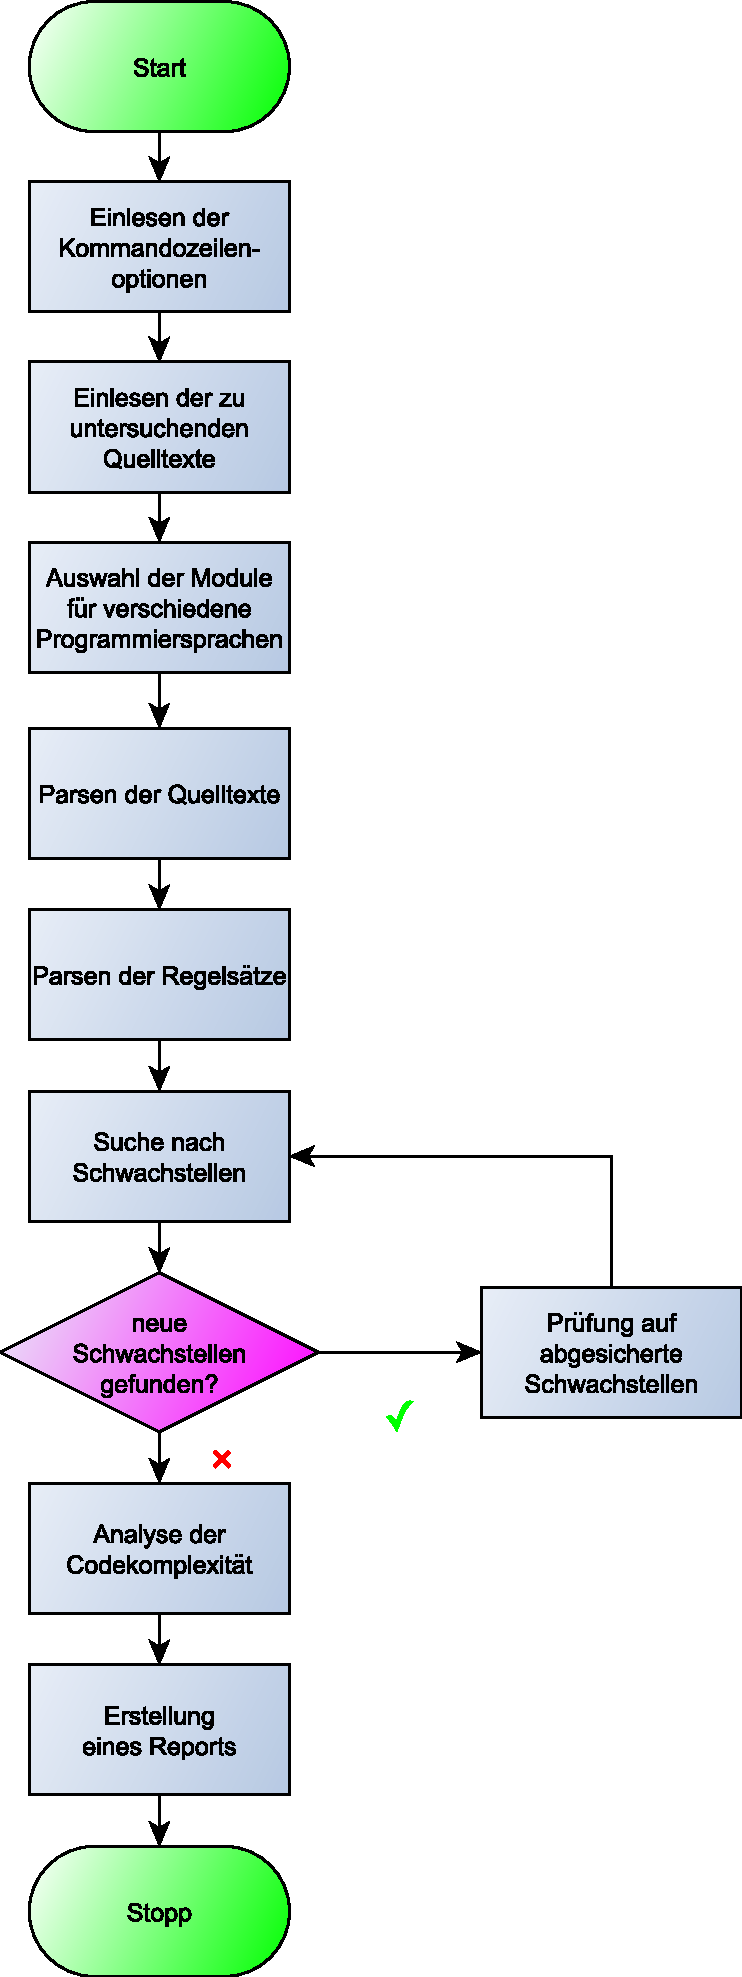
\includegraphics[max height=\textheight, max width=\textwidth]{Programmablaufplan.pdf}
            \captionbelow{Programmablaufplan (grob)}\label{fig:Programmablaufplan}
        \end{figure}
        Der grobe Programmablauf kann dem Programmablaufplan aus
        \vref{fig:Programmablaufplan} entnommen werden.

        Zuerst werden die Kommandozeilenoptionen des Programms eingelesen.
        Hier kann der Anwender auswählen,
        welche Dateien untersucht werden sollen,
        ob er die Auswahl des Moduls für die Untersuchung unerkannter Dateiformate erzwingen will
        (vergleiche
        \vref{Vergleich Dateiformaterkennung}) sowie
        welches Ausgabeformat genutzt werden soll.

        Hiermit soll es einem Anwender ermöglicht werden,
        beliebige Dateien oder
        auch komplette Verzeichnisse mit Quelltexten auf Schwachstellen zu untersuchen.

        Nach der Auswahl der zu untersuchenden Dateien muss anschließend das Framework herausfinden,
        welche Module für die Untersuchung infrage kommen.
        Zu diesem Zweck wird entweder die Dateiendung oder
        die
        \hyperref[Magische Zahl]{Magische Zahl} verwendet.
        Ein Vergleich dieser beiden Methoden findet sich in
        \vref{Vergleich Dateiformaterkennung}.

        Da allerdings beide Erkennungsmethoden ihre Schwächen haben,
        kann die Erkennung auch durch eine Heuristik oder
        den Benutzer selber festgelegt werden.

        Anschließend müssen die Quelltexte anhand von Grammatiken,
        welche in den Modulen beschrieben sind,
        geparst werden,
        um eine für das Framework nutzbare Repräsentation des Quelltextes zu erhalten.

        Bei der Erstellung dieser Repräsentation ist es wichtig,
        dass sämtliche Funktionsnamen erhalten bleiben,
        da im späteren Verlauf anhand derer erkannt wird,
        ob verwundbare Funktionen,
        Benutzereingaben und
        Absicherungen vorhanden sind und
        wie sie miteinander in Beziehung stehen.

        Um diese Repräsentation auf Schwachstellen untersuchen zu können,
        müssen vordefinierte Regelsätze genutzt werden,
        wie sie in
        \vref{Erstellung Regelsaetze} beschrieben werden.

        Anschließend kann die Suche nach Schwachstellen beginnen,
        wie in
        \vref{Auffinden verwundbarer Funktionen} beschrieben wird.

        Hierbei ist es notwendig,
        die Quelltexte mindestens zweimal zu untersuchen,
        da eine Untersuchung zum Beispiel im ersten Durchlauf eine Schwachstelle finden kann,
        diese allerdings durch eine andere Funktion indirekt abgesichert wird,
        sodass diese zweite Funktion als zusätzliche absichernde Funktion hinzugefügt werden muss,
        bevor die Funktion neu untersucht und
        die Schwachstelle als abgesichert markiert werden kann.

        Da diese indirekte Absicherung allerdings nicht den Best Practices der sicheren Programmierung entspricht,
        senkt sie das erkannte Risiko weniger als eine direkte Absicherung
        (vergleiche
        \vref{Definition von Absicherungen}).

        Da,
        wie in
        \vref{Implikationen für die statische Analyse} bewiesen,
        keine 100\,\%ige Erkennung aller Schwachstellen mittels statischer Analyse möglich ist,
        wird zusätzlich durch eine Analyse der Codekomplexität auf Funktionen hingewiesen,
        welche sehr komplex sind und
        daher mit höherer Wahrscheinlichkeit Fehler enthalten als andere Funktionen.

        Zum Abschluss wird aus den gesammelten Daten ein Bericht in einem vom Benutzer gewählten Format erstellt und
        das Programm endet.

    \section{Anforderungen}
        Ziel des Frameworks ist es,
        bei der Suche nach Sicherheitslücken in Quelltexten zu helfen.

        Hierzu müssen zum einen die Dateiformate korrekt erkannt werden,
        zum anderen müssen aber auch Module vorhanden sein,
        welche zur Analyse der jeweiligen Dateien dienen und
        anhand von Regelsätzen Sicherheitslücken erkennen.

        Hierbei ist es wichtig,
        dass die Erstellung von Regelsätzen und
        -- nach Möglichkeit
        -- auch die Erstellung neuer Module für den Endanwender möglichst einfach ist,
        da im Rahmen dieser Masterarbeit aufgrund des zeitlichen Rahmens natürlich nur ein begrenzter Umfang an Modulen und
        Regelsätzen erstellt werden kann.

        Da im Rahmen dieser Masterarbeit ein komplett neues Framework erstellt wird,
        wird die Optimierung der Geschwindigkeit oder
        das Abdecken sämtlicher Kategorien von Schwachstellen als nachrangig betrachtet.

        Vorrangig wird versucht,
        den Programmiercode möglichst gut leserlich und
        einfach erweiterbar zu gestalten sowie
        die Module und
        Regelsätze in einer einfachen und
        gleichzeitig ausreichend mächtigen Form zu erstellen.

        Hierdurch sollte es möglich sein,
        das Framework und
        die enthaltenen Regeln im eigenen Betrieb laufend zu erweitern und
        eigene Regelsätze anhand der individuellen Erfahrungen und
        Anforderungen anzulegen.

        Hiermit sollte es möglich sein,
        ein Framework zu erstellen,
        welches als Universallösung etabliert und
        ständig weiterentwickelt werden kann,
        ohne dass eine aufwendige Einarbeitung in immer neue Produkte erforderlich wird,
        weil die bestehenden Produkte veraltet sind und
        keine Updates mehr angeboten werden.

    \section{Anwendungsgebiete}\label{Anwendungsgebiete}
        Mit einer statischen Codeanalyse wird der komplette Code eines Programms gescannt,
        ohne dass er dabei ausgeführt werden muss.

        Somit ist es möglich,
        sogar Schwachstellen in kaum genutzten Codestellen zu finden,
        die aufgrund schwerer Erreichbarkeit in einem üblichen Penetration Test unter Umständen übersehen würden.

        Hierdurch können Sicherheitslücken nicht nur schnell gefunden werden,
        sondern ein entsprechender Scan kann auch automatisiert eingebunden werden,
        wodurch Zeit und
        Entwicklungskosten gegenüber einer manuellen Prüfung gespart werden.

        Auf der anderen Seite kann eine statische Codeanalyse nicht sämtliche Fehler in einem Quelltext finden
        (vergleiche
        \vref{Implikationen für die statische Analyse}),
        sodass die statische Analyse als Ergänzung zur manuellen Analyse von Quelltexten und
        einem Penetration Test eingesetzt werden sollte.

        Weiterhin findet das entwickelte Framework Sicherheitslücken unabhängig von Schutzmechanismen des Betriebssystems,
        was bedeutet,
        dass nicht jede Lücke,
        die gefunden wird,
        automatisch auch auf allen betroffenen Systemen ausnutzbar ist,
        sofern das Betriebssystem einen entsprechenden Schutzmechanismus einsetzt.

        Da allerdings zum einen diese Schutzmechanismen nicht auf allen Systemen installiert und
        aktiviert sind und
        zum anderen Sicherheitslücken teilweise auch auf ein tiefer liegendes Problem,
        wie ein mangelndes Verständnis des Entwicklers für sichere Programmierung oder
        Unachtsamkeit,
        hinweisen können,
        werden vom Framework lieber mehr nicht"=ausnutzbare Lücken entdeckt,
        als ausnutzbare zu übersehen.

        Durch die entstehende erhöhte Anzahl an False Positives bei gleichzeitig sinkender Anzahl False Negatives,
        wird ein Einsatz in Kombination mit dem OWASP DefectDojo\cite{Anderson2018} oder
        ähnlichen Projekten empfohlen.

    \section{Marktanalyse}
        Bei jeder Neuentwicklung ist es wichtig zu betrachten,
        welche Produkte derzeit erhältlich sind und
        wie sie sich von den eigenen Ideen unterscheiden,
        um festzustellen,
        ob sich die Neuentwicklung lohnt oder
        ob es sinnvoller ist,
        in eines der bestehenden Produkte zu investieren.

        Aus diesem Grund wurde auch vor Beginn der Entwicklung dieses Frameworks eine Marktanalyse durchgeführt.

        Das Ergebnis dieser Analyse brachte allerdings hervor,
        dass es nur wenige direkt vergleichbare Produkte gibt und
        diese teilweise entweder nicht mehr weiter entwickelt werden oder
        einen zu engen Fokus haben und
        somit eine Einbindung von mehreren Produkten gleichzeitig notwendig wäre,
        was aufgrund des Aufwands,
        allein einen statischen Codescanner in der Entwicklungswerkzeugkette zu etablieren,
        schnell zu Ablehnung seitens der Anwender führen kann.

        \subsection{Vergleichbare Produkte}
            Zwei Produkte,
            die dem Ziel dieses Frameworks vergleichsweise nah kommen,
            werden im Folgenden näher betrachtet und
            dabei wird aufgezeigt,
            aus welchem Grund eine Neuentwicklung notwendig ist.

            Hiermit soll keineswegs die Qualität dieser Produkte angezweifelt werden,
            welche mitunter weit längere Entwicklungszeiten hatten und
            sich in der Praxis gut bewährt haben.

            Stattdessen soll gezeigt werden,
            welche Schwachstellen eine größere Verbreitung verhindern und
            wie diese behoben werden können.

            \subsubsection{PyT}
                Das PyT-Projekt
                (kurz für
                \foreignquote{english}{Python Taint}) ist ein aus einer Masterarbeit\cite{Micheelsen2016} entstandener,
                statischer Codescanner für Webanwendungen,
                welcher Command Injections,
                \gls{SSRF},
                \gls{SQL} Injections,
                \gls{XSS},
                Directory Traversal und weitere Lücken erkennen kann.

                Die Arbeit ist zwar eine große Inspiration für die Erstellung der vorliegenden Masterarbeit,
                da sie sich jedoch auf die Schwachstellenerkennung in Webframeworks beschränkt,
                unterliegt sie einigen dramatischen Einschränkungen,
                die einer hohen Verbreitung entgegenstehen.

                Zum Ersten werden derzeit nur zwei Webframeworks,
                Flask\cite{Ronacher2018} und
                Django\cite{DSF2018},
                von dem Projekt untersucht.

                Weiterhin implementiert das Projekt keinen eigenen Parser
                (vergleiche
                \vref{Aufbau eines Parsers}),
                sondern nutzt das Python"=Modul
                \texttt{ast}\cite{PSF2018},
                welches Teil der Python"=Standardbibliothek ist und
                lediglich die Untersuchung von Python"=Code ermöglicht.

                Da hierdurch die Untersuchung anderer Programmiersprachen
                -- wie
                \gls{PHP}
                -- unmöglich wird und
                auch keine Untersuchung von beliebigen weiteren Python"=Projekten geplant ist,
                ist der Rahmen des Projekts zu klein,
                um eine weite Verbreitung zu ermöglichen.

                Auf der anderen Seite erlaubt dieser enge Rahmen natürlich eine Spezialisierung und
                sehr gute Qualität der Analyse.
                Diese könnte allerdings auch mit entsprechend guten Regeln in einem allgemeiner gehaltenen Projekt erreicht werden.

                Durch die gute Dokumentation des Projekts und
                die vielen allgemein verwendbaren guten Ansätze dient es allerdings im weiteren Verlauf dieser Ausarbeitung häufig als Inspiration und
                es wird auf den Ansätzen und Ergebnissen aufgebaut.

            \subsubsection{RATS}
                RATS
                (kurz für
                \foreignquote{english}{Rough Auditing Tool for Security})\cite{SecureSoftware2013} ist ein statischer Schwachstellenscanner für C,
                C++,
                Perl,
                \gls{PHP},
                Python und
                Ruby.

                Er unterstützt die Prüfung auf häufige Schwachstellen wie Buffer Overflows,
                \gls{TOCTOU} und
                Race Conditions.

                RATS benutzt hierfür einen eigenen Parser
                (vergleiche
                \vref{Aufbau eines Parsers}),
                um eine gute Erkennung zu gewährleisten.

                Leider wird RATS bereits seit dem 31.~Dezember 2013 nicht mehr weiterentwickelt und
                die Regelsätze zur Erkennung von Schwachstellen sind direkt in den C"=Code integriert,
                sodass eine Erweiterung der Regeln für Anwender nur mit viel Einarbeitungszeit
                in den Quelltext von RATS verbunden ist.

                RATS kommt daher den Zielen dieser Masterarbeit bereits sehr nahe,
                durch die Integration der Schwachstellendefinitionen in den Quelltext wird allerdings auch hier die weitere Verbreitung erschwert.

                Da außerdem das Projekt nicht mehr aktiv weiterentwickelt wird,
                ist es höchstens eine Frage der Zeit,
                bis der Parser nicht mehr in der Lage ist,
                neue Versionen der oben aufgelisteten Programmiersprachen korrekt zu untersuchen.

    \section{Auffinden verwundbarer Funktionen}\label{Auffinden verwundbarer Funktionen}
        Um verwundbare Funktionen in Quelltexten zu finden,
        gibt es verschiedene Ansätze,
        die nachfolgend vorgestellt und
        miteinander verglichen werden.

        Hierdurch ist es möglich,
        die Vor"= und
        Nachteile der einzelnen Ansätze darzustellen und
        einen Ansatz zu wählen,
        der sowohl
        mit vertretbarem Implementierungsaufwand,
        als auch mit ausreichender Qualität Schwachstellen im Code aufdecken kann.

        Im Folgenden werden daher drei Ansätze vorgestellt und
        miteinander verglichen.

        Leider unterliegen alle vorgestellten Ansätze einigen Einschränkungen,
        die zu Anfang besprochen werden,
        um die Grenzen der statischen Analyse aufzuzeigen.

        \subsection{Allgemeine Einschränkungen}\label{Allgemeine Einschränkungen}
            Bei der statischen Analyse von Code ist es niemals möglich,
            mit 100\,\%iger Sicherheit sämtliche Schwachstellen im Code zu finden.

            Dieses Ergebnis liegt zum einen am Satz von Rice,
            wie in
            \vref{Satz von Rice} nachvollzogen werden kann.

            Zum anderen müssen allerdings auch die Regelsätze zur Erkennung von Schwachstellen von Menschen erstellt werden,
            sodass es immer möglich ist,
            dass Schwachstellen zwar theoretisch erkannt werden könnten,
            der Regelsatz zur Erkennung aber entweder nicht existiert oder
            fehlerhaft bzw.\ zu spezialisiert ist,
            sodass im konkreten Fall die Erkennung trotzdem fehlschlägt.

            Weiterhin darf die Analyse nicht zu lange dauern,
            um die Entwicklung nicht zu sehr aufzuhalten,
            da ansonsten davon auszugehen ist,
            dass die Anwender den Scan nicht regelmäßig durchführen würden.

            Die statische Analyse ist daher auch zeitlich eingeschränkt,
            wobei diese Grenze nicht fest definierbar ist,
            da es für das eine Unternehmen möglich ist,
            den Scan über Nacht unbeaufsichtigt laufen zu lassen,
            wohingegen ein anderes einen Scan nach jedem Commit auf den Server anstrebt.

            Es ist allerdings möglich,
            nur einzelne Dateien zu scannen,
            welche durch einen Commit geändert wurden,
            weshalb, wie bereits angesprochen,
            das Framework für die erste Entwicklung nicht auf schnelle Ausführungszeit optimiert wird.

            Da es bei der Suche nach Sicherheitslücken in der Regel wichtiger ist,
            dass mehr tatsächliche Sicherheitslücken gefunden werden,
            als dass weniger falsche Sicherheitslücken entdeckt werden,
            wird dabei versucht,
            eine möglichst gute regelbasierte Erkennung zu ermöglichen,
            die allerdings eine geringere Komplexität bei der Erstellung von Regelsätzen
            -- und
            damit eine niedrigere Schwelle zur Erstellung und
            Anpassung eigener Regeln durch den Benutzer
            -- auf Kosten der Vermeidung von False Positives vorzieht.

            Diese Abwägung erscheint sinnvoll,
            da die Bewertung der Schwachstellen ohnehin später von Experten vorgenommen werden muss und
            diese,
            wie in
            \vref{Anwendungsgebiete} beschrieben,
            das Framework mit weiteren Projekten kombinieren können,
            um Reports zu speichern und
            damit False Positives in nachfolgenden Reports nicht mehr aufzuführen.

        \subsection{Vergleich verschiedener Ansätze}
            Im Folgenden werden verschiedene Ansätze zur statischen Analyse von Quelltexten verglichen.

            Dabei wird aufgezeigt,
            welche Ansätze grundsätzlich existieren,
            wie effektiv sie sind, und
            wie aufwendig der spätere Einsatz wäre.

            Im Anschluss werden die Ansätze miteinander verglichen und
            eine Entscheidung über den für diese Masterarbeit zu wählenden Ansatz begründet.

            Es ist hierbei wichtig festzustellen,
            dass es keinen perfekten Ansatz für die Suche nach Schwachstellen in Quelltexten gibt,
            sodass immer eine Abwägung zwischen guter Erkennung von Schwachstellen,
            Geschwindigkeit und
            Komplexität des Ansatzes getroffen werden muss.

            Auch kann die folgende Auflistung keine vollständige Liste darstellen,
            da einige Ansätze,
            wie zum Beispiel das Übersetzen der Quelltexte in ausführbaren Code und
            ein anschließendes Testen mit zufälligen Eingaben,
            sogenanntes
            \foreignquote{english}{Fuzzing},
            nicht als für diesen Zweck geeignete Methode angesehen wird,
            da hiermit die Erkennung zufallsbasiert ist und
            nicht nur Schwachstellen unerkannt bleiben können,
            sondern erkannte Fehler auch keine Rückschlüsse darüber zulassen,
            ob es sich um eine Schwachstelle handelt und
            wie diese behoben werden könnte.

            Weitere Analysemethoden,
            die auf die Erkennung von Schwachstellen nicht mehr in den Quelltexten,
            sondern in den Binärdateien zielen,
            bleiben beim folgenden Vergleich aus diesem Grund unberücksichtigt.

            \subsubsection{Einfache Stringsuche}\label{Einfache Stringsuche}
                Eine einfache Stringsuche ist die wohl am leichtesten implementierbare Methode,
                um verwundbare Funktionen und
                Angriffsmuster in Quelltexten zu erkennen.

                Es reicht hierfür ein regulärer Ausdruck,
                durch den zum Beispiel ungefilterte
                \gls{SQL}"=Abfragen wie in
                \vref{Beispiel eines verwundbaren PHP-Skripts} erkannt werden können.
                Für diesen Fall könnte ein Ausdruck der folgenden Form zur Erkennung in
                \gls{PHP}"=Skripten dienen:

                \lstinline@mysql_query\((["'])SELECT .+ FROM .+ WHERE .+(?:\=|\s+I?LIKE\s+|<>|>=?|<=?).+\1\)@

                Mit diesem Muster wird der fixe String
                \enquote{mysql\_query(} gefolgt von entweder einem doppelten oder
                einfachen Anführungszeichen gesucht,
                wiederum gefolgt von dem fixen String
                \enquote{SELECT },
                einem oder mehreren beliebigen Zeichen,
                dem fixen String
                \enquote{ FROM },
                wieder einem oder mehreren beliebigen Zeichen,
                \enquote{ WHERE } und
                anschließend beliebigen Zeichen gefolgt von einem Vergleichsoperator,
                einem oder mehreren weiteren beliebigen Zeichen und
                einem zweiten doppelten oder
                einfachen Anführungszeichen,
                je nachdem,
                welches Zeichen am Anfang gefunden wurde.

                Wie man allerdings sehen kann,
                werden derartige reguläre Ausdrücke schnell unübersichtlich,
                sodass selbst in solchen vergleichsweise einfachen Fällen eine Visualisierung,
                wie in diesem Fall mittels Regexper\footnote{\href{https://regexper.com}{https://regexper.com}} erstellt und
                in \vref{fig:SQLi-Regex} zu sehen,
                notwendig ist,
                um den Ausdruck zu verstehen.

                \begin{figure}[htp]
                    \centering%
                    \includegraphics[max height=\textheight, max width=\columnwidth]{SQLi-Regex.png}
                    \captionbelow{Regulärer Ausdruck zum Finden von SQL Injections}\label{fig:SQLi-Regex}
                \end{figure}

                Selbst dieser Ausdruck stößt allerdings schnell an seine Grenzen,
                da auch ungültige
                \gls{SQL}"=Anweisungen erkannt werden.
                Weiterhin können
                -- wenn die Suche zeilenübergreifend stattfindet,
                wie es in einigen Sprachen standardmäßig der Fall ist und
                in anderen über das
                \foreignquote{english}{multiline}"=Flag eingeschaltet werden kann
                -- teilweise mehrere Zeilen zusammen einen Treffer ergeben,
                der alleine nie im Programmcode vorkommt.

                Auf der anderen Seite könnten
                \gls{SQL}"=Abfragen im Code über mehrere Zeilen mit Stringumbrüchen geschrieben sein,
                was wiederum von der Abfrage oben nicht unterstützt wird und
                somit anfällige Abfragen übersehen könnte.

                Auch ist es hiermit nicht möglich,
                zwischen Code und Kommentaren zu unterscheiden,
                sodass eine größere Anzahl von False Positives entsteht.

                Es wäre daher wünschenswert,
                einen Ansatz zu finden,
                welcher die Funktion anhand des Namens erkennt,
                gleichzeitig aber auch in der Lage ist,
                Parameter der Anweisung zu erkennen und
                damit festzustellen,
                ob eine Variable in den Code eingefügt wurde oder
                ob es sich um ein \foreignquote{english}{Prepared Statement},
                also eine von der Datenbank vorbereitete Abfrage,
                welche keinen zusätzlichen Code mehr ausführen kann und
                somit vor \gls{SQL}"=Injection"=Angriffen geschützt ist,
                handelt.

            \subsubsection{Erstellung eines Parsers}
                Die Erstellung eines Parsers ist im Vergleich zur Stringsuche weitaus aufwendiger,
                da zuerst die Grammatik der Sprache untersucht werden muss,
                anhand derer anschließend nach verwundbaren Funktionen gesucht werden kann.
                Es handelt sich also so gesehen um eine Erweiterung der Stringsuche.

                Sie hat allerdings den Vorteil,
                dass automatisch zwischen Code und
                Kommentaren unterschieden wird,
                wodurch die Anzahl der False Positives sinkt.

                Weiterhin können hiermit zusammenhängende Zeilen aufgelöst und
                als einzelne Anweisung erkannt und
                verarbeitet werden.

                Auch bei der Erstellung eines Parsers ist es erforderlich,
                verwundbare Funktionen zu erkennen,
                sodass auch hier reguläre Ausdrücke notwendig sind.

                Im Vergleich zur einfachen Stringsuche können die Ausdrücke allerdings weitaus einfacher sein,
                da durch den Parser bereits viele Ausdrücke normalisiert und
                in ihre Bestandteile aufgelöst wurden.

                Leider können durch den Parser wieder nur Muster erkannt werden,
                es kann nicht geprüft werden,
                ob eine Ausführung mit verschiedenen Daten zu korrekten Ergebnissen führt oder
                ob es vielleicht sogar zu einem Überschreiben von Daten im Speicher kommt.

            \subsubsection{Analyse durch symbolische Ausführung}\label{Analyse durch symbolische Ausführung}
                Bei der symbolischen Ausführung wird das Programm von einem Interpreter simuliert,
                wobei allerdings keine echten Werte als Eingaben verwendet werden,
                sondern lediglich Symbole.\cite[5]{Hicks2013}

                Nachdem der Interpreter das Programm komplett durchlaufen hat,
                wobei für sämtliche möglichen Verzweigungen neue Symbole erzeugt wurden,
                wird ein Constraint Solver
                -- also ein Programm,
                welches versucht,
                das Erfüllbarkeitsproblem
                (SAT) für sämtliche Verzweigungen zu lösen
                -- eingesetzt,
                um sämtliche möglichen Pfade durch das Programm zu erkennen.

                Eines der Hauptprobleme hierbei ist,
                dass es aufgrund der Vielzahl an möglichen Pfaden durch ein Programm zu einer sogenannten Pfadexplosion kommen kann.\cite[9]{Hicks2013}

                Weiterhin wäre es notwendig,
                nicht nur einen Parser,
                sondern auch einen Interpreter für jede Programmiersprache zu erstellen,
                welcher die symbolische Ausführung ermöglicht.

                Zwar ist die Rechengeschwindigkeit heute weit besser,
                als in den Anfangszeiten der symbolischen Ausführung,
                da es sich bei dem Erfüllbarkeitsproblem allerdings um ein
                \gls{NP}"=vollständiges Problem handelt
                -- was nach aktuellem Stand der Forschung bedeutet,
                dass kein effizienter Algorithmus zum Lösen des Problems existiert
                -- kann sie auch heute noch nicht uneingeschränkt für die Suche nach Schwachstellen empfohlen werden.

            \subsubsection{Vergleich der Ansätze und Begründung der Entscheidung}
                Von den vorgestellten Ansätzen erscheint die Erstellung eines Parsers am vielversprechendsten.

                Hierbei kommt es zu weniger False Positives und
                -- was noch viel wichtiger ist
                -- zu weniger False Negatives durch nicht korrekt erkannte Funktionen als bei der Stringsuche,
                gleichzeitig kommt es aber nicht zu einer Pfadexplosion und
                der Implementierungsaufwand hält sich im Rahmen.

                Durch die Erstellung eines Parsers ist es möglich,
                verwundbare Funktionen gezielt zu suchen und
                dabei gleichzeitig die Schwächen einer zu groben Suche zu vermeiden.

                Da der Ansatz der symbolischen Ausführung allerdings auch seine Vorzüge hat,
                scheint es sinnvoll,
                diesen in modifizierter Form ebenfalls in das zu erstellende Framework aufzunehmen.

                Konkret sollen bei Verzweigungen grundsätzlich sämtliche Möglichkeiten getestet werden,
                um zu erkennen,
                ob eine Schwachstelle im Quelltext existiert und
                woher die Eingaben für diese Schwachstelle kommen.
                Vergleiche hierzu auch
                \vref{Vereinfachungen und deren Auswirkungen auf die Qualität der Analyse}.

    \section{Aufbau eines Parsers}\label{Aufbau eines Parsers}
        Bei einem Parser handelt es sich um ein Programm,
        welches eine Eingabe in Form eines Quelltextes zerlegt und
        für die Weiterverarbeitung aufbereitet.

        Mit anderen Worten ist der Parser dafür verantwortlich,
        aus dem für Menschen lesbaren Quelltext eine Repräsentation zu schaffen,
        welche vom Computer algorithmisch verarbeitet werden kann.

        Somit kommt dem Parser gerade in Bezug auf die statische Analyse eine sehr wichtige Rolle zu,
        da die Qualität des Parsers maßgeblich bestimmt,
        welche Daten im Anschluss überhaupt überprüft werden können und
        wie diese miteinander in Zusammenhang stehen.

        Wenn der Parser zum Beispiel eine Struktur im Code nicht richtig erkennt,
        so gibt es keine Möglichkeiten,
        diese Erkennung nachträglich noch hinzuzufügen.

        Auf der anderen Seite muss der Parser allerdings eine Vereinfachung des Codes repräsentieren,
        da für den Programmablauf unnötige Elemente aus dem Quelltext entfernt und
        Konstrukte vereinheitlicht werden.

        Da außerdem nicht in jedem Fall garantiert werden kann,
        dass die vom Framework ermittelten Repräsentationen dem entsprechen,
        was ein Compiler entwerfen würde und
        es auch schon zu Sicherheitslücken durch übereifrige Optimierungen von Compilern gekommen ist,\cite{Wang2012}
        kann nicht garantiert werden,
        dass durch diesen Ansatz sämtliche Sicherheitslücken gefunden werden,
        welche später im lauffähigen Programm auftreten könnten.

        Eine Annäherung durch möglichst enge Orientierung des Parsers am Standard ist dabei die beste Voraussetzung,
        um eine möglichst gute Erkennung zu garantieren.

        Ein Parser besteht dabei aus mehreren Teilen,
        die nachfolgend kurz erläutert werden.

        Der Großteil der hier vorgestellten Definitionen basiert auf dem Vortrag
        \foreignquote{english}{So you want to write an interpreter?} von Alex Gaynor.\cite{Gaynor2013}

        \subsection{Der Lexer}
            Ein Lexer ist ein Programm,
            welches eine Eingabe in eine Liste von Tokens übersetzt.
            Dieser Prozess wird als die
            \enquote{lexikalische Analyse} bezeichnet.

            Jeder Token stellt dabei eine grundlegende syntaktische Komponente der Programmiersprache dar.
            So sind zum Beispiel ein einfaches
            \verb|+| oder
            auch ein
            \verb|<=| in vielen Programmiersprachen gültige Tokens.

            Leerzeichen,
            Zeilenumbrüche und
            Tabs,
            aber auch Kommentare werden häufig von der lexikalischen Analyse verworfen,
            da sie keinen syntaktischen Unterschied ausmachen.\cite[38]{Watson2017}

            Als Beispiel soll der folgende C"=Code dienen:\cite[38]{Watson2017}

            \begin{lstlisting}[caption={Beispiel C-Code}, label={lst:Beispiel_C_Code}, gobble=16,
                language=C]
                while (i <= 100) {
                    tot += a[i]; /* form vector total */
                    i++;
                }
            \end{lstlisting}

            Die lexikalische Analyse würde hieraus folgende Tokens generieren:

            \begin{itemize}
                \item \verb|while| (RESERVEDWORD)
                \item \verb|(| (LPAREN)
                \item \verb|i| (IDENTIFIER)
                \item \verb|<=| (LESS\_EQUAL)
                \item \verb|100| (INTEGERCONSTANT)
                \item \verb|)| (RPAREN)
                \item \verb|{| (LBRACE)
                \item \verb|tot| (IDENTIFIER)
                \item \verb|+=| (PLUS\_EQUALS)
                \item \verb|a| (IDENTIFIER)
                \item \verb|[| (LSQUARE)
                \item \verb|i| (IDENTIFIER)
                \item \verb|]| (RSQUARE)
                \item \verb|;| (SEMICOLON)
                \item \verb|i| (IDENTIFIER)
                \item \verb|++| (PLUSPLUS)
                \item \verb|;| (SEMICOLON)
                \item \verb|}| (RBRACE)
            \end{itemize}

            In Klammern wurden hierbei Bezeichnungen für die Gruppe angegeben,
            zu denen das Token gehört.

            So kann man zum Beispiel erkennen,
            dass es sich sowohl bei dem Token
            \verb|i|,
            als auch bei dem Token
            \verb|tot| und
            dem Token
            \verb|a| um Variablen handelt.

            Hierbei ist es wichtig zu beachten,
            dass der Lexer keinerlei Prüfung auf Gültigkeit der
            \texttt{while}"=Schleife vornimmt.
            Diese Aufgabe würde
            später dem Interpreter oder
            Compiler zukommen.

            Da ein solcher allerdings für die statische Analyse nicht erstellt wird,
            entfällt hier eine aufwendige Prüfung auf syntaktische Korrektheit des gesamten Programms und
            es findet lediglich eine Prüfung auf gültige Tokens statt.

            Um den Lexer dabei möglichst robust zu gestalten,
            ist es im Framework möglich,
            ungültige Tokens zu ignorieren.

            Damit sinkt zwar die Qualität der Eingabe und
            damit auch die Qualität der Schwachstellenerkennung insgesamt,
            allerdings bringen auch neue Sprachkonstrukte den Parser hierdurch nicht direkt zum Absturz,
            wenn kein entsprechendes Update der Module vorgenommen wurde.

            Um neue Tokens hinzuzufügen,
            werden reguläre Ausdrücke verwendet,
            durch welche die allgemeine Form eines Tokens beschrieben wird.

            Dadurch,
            dass die Tokens die kleinsten Bausteine des Quelltextes sind,
            lässt sich somit in einer Art Divide and Conquer eine Vereinfachung der benötigten regulären Ausdrücke ermöglichen.

        \subsection{Der eigentliche Parser}
            Der Parser bekommt als Eingabe die Ausgabe des Lexers und
            versucht,
            die Struktur des Codes zu ermitteln.
            Zu diesem Zweck baut der Parser einen sogenannten
            \foreignquote{english}{Parse Tree} auf.

            Hierfür wird typischerweise entweder ein Top"=Down"=Ansatz
            (vergleiche
            \vref{Top-Down}) oder
            ein Bottom"=Up"=Ansatz
            (vergleiche
            \vref{Bottom-Up}) genutzt.

            Beide Ansätze sollen nachfolgend kurz erklärt werden,
            um ein Verständnis für die Funktionsweise des eingesetzten Parsers sowie
            mögliche Schwierigkeiten bei der Implementierung besser abschätzen zu können.

            Da allerdings der Fokus dieser Ausarbeitung nicht Compilerbau ist,
            werden beide Verfahren nur kurz erklärt.
            Eine ausführlichere Erklärung kann zum Beispiel in
            \cite[77]{Watson2017} gefunden werden.

            \subsubsection{Top-Down}\label{Top-Down}
                Ein Top"=Down"=Parser startet bei einem einzigen Knoten,
                welcher mit dem Startsymbol gekennzeichnet ist.
                Anschließend baut er nacheinander von links nach rechts Unterbäume auf.

                Zur Veranschaulichung soll folgendes Beispiel genutzt werden:

                Der Ausdruck
                \verb|1 * 0 + 1| soll ausgewertet werden.
                Folgende Regeln existieren in der Grammatik:

                \begin{lstlisting}[caption={Grammatik einer einfachen arithmetischen Sprache}, gobble=20]
                    <expr> ::= <term> | <expr> + <term>
                    <term> ::= <digit> | <term> * <digit>
                    <digit> ::= 0 | 1
                \end{lstlisting}
                Die Auswertung könnte nun wie in \vref{fig:Top-Down} aussehen.

                \begin{figure}[htp]
                    \centering%
                    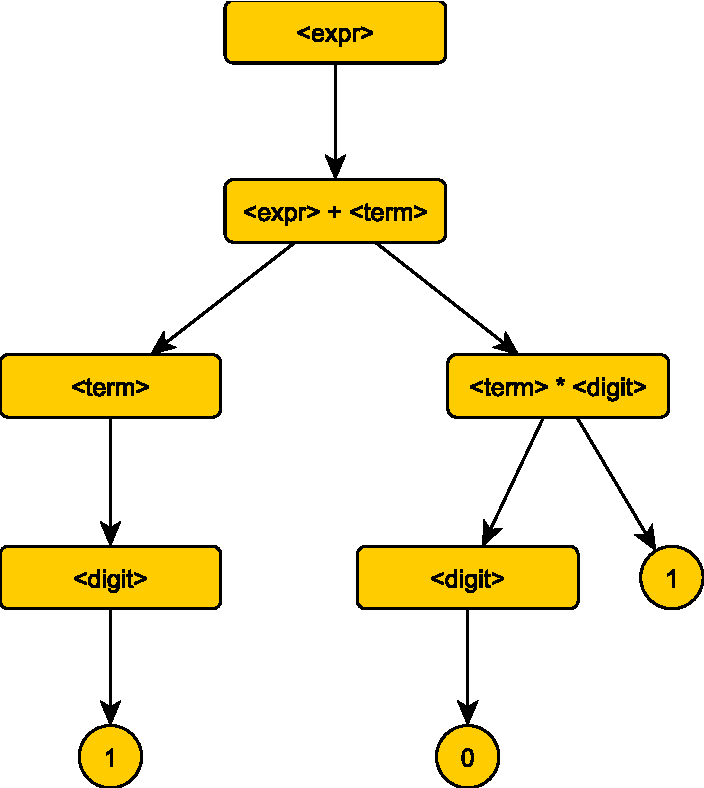
\includegraphics[max height=\textheight, max width=\textwidth]{Top-Down.pdf}
                    \captionbelow{Aufbau eines Parse Trees mit Top-Down-Ansatz}\label{fig:Top-Down}
                \end{figure}

                Es ist hierbei wichtig zu beachten,
                dass die Entscheidung,
                am Anfang nicht die Seite
                \lstinline{<expr> ::= <term>},
                sondern
                \lstinline{<expr> ::= <expr> + <term>} auszuwerten,
                im Normalfall über Prioritätsdefinitionen geregelt werden muss,
                die allerdings für diese Veranschaulichung übersprungen werden.

            \subsubsection{Bottom-Up}\label{Bottom-Up}
                Im Gegensatz zum Top"=Down"=Ansatz startet der Bottom"=Up"=Ansatz nicht mit dem Startsymbol,
                sondern mit dem ersten Token der Eingabe.
                Anschließend werden solange Tokens ausgewertet,
                bis das Startsymbol erreicht ist.

                Zur Veranschaulichung soll auch hier wieder der Ausdruck aus
                \vref{Top-Down} dienen.
                Dieses Mal könnte die Auswertung
                wie in
                \vref{fig:Bottom-Up} aussehen.

                \begin{figure}[htp]
                    \centering%
                    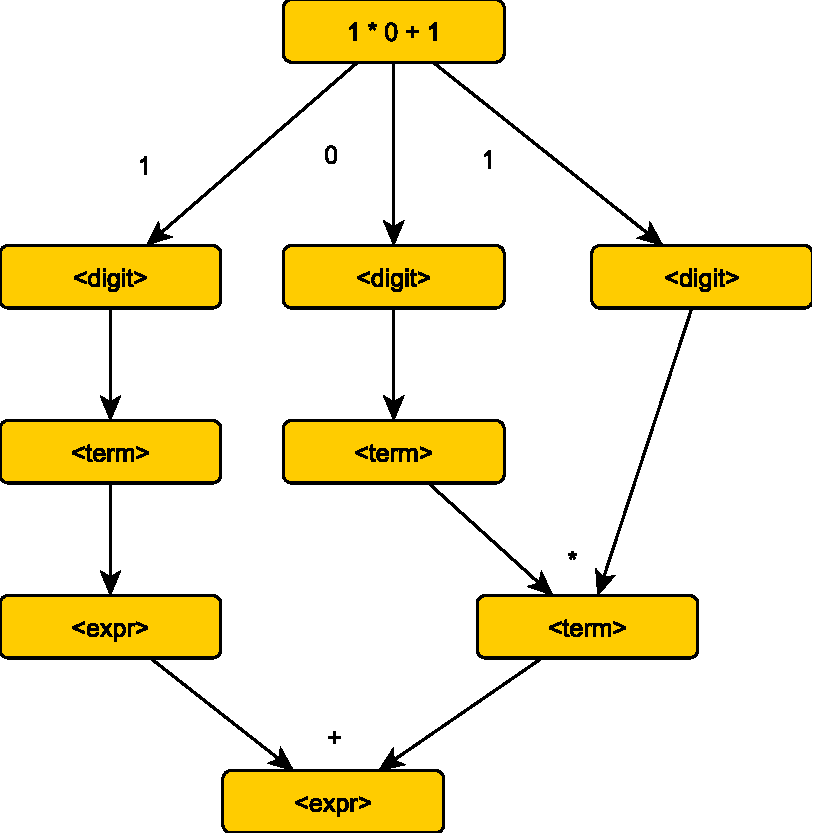
\includegraphics[max height=\textheight, max width=\textwidth]{Bottom-Up.pdf}
                    \captionbelow{Aufbau eines Parse Trees mit Bottom-Up-Ansatz}\label{fig:Bottom-Up}
                \end{figure}

        \subsection{Der AST}\label{Der AST}
            Bei einem
            \gls{AST} handelt es sich um eine weitere Abstraktion über dem vom Parser generierten
            \foreignquote{english}{Parse Tree}.
            Hierbei werden sämtliche Bestandteile entfernt,
            welche den Ablauf von Reduktionen im Baum oder
            sonstige Syntax"=Eigenheiten widerspiegeln.\cite[26]{Watson2017}

            Im Vergleich zu
            \vref{fig:Top-Down} könnte ein entsprechender
            \gls{AST} zum Beispiel
            wie in
            \vref{fig:AST} aussehen.

            \begin{figure}[htp]
                \centering%
                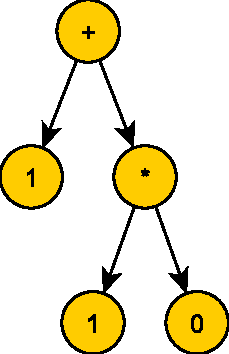
\includegraphics[max height=\textheight, max width=\textwidth]{AST.pdf}
                \captionbelow{Beispiel eines AST}\label{fig:AST}
            \end{figure}

            Wie man hieran sehen kann,
            wurden sämtliche Gruppenzugehörigkeiten entfernt und
            es bleibt nur noch die reine Programmlogik in einem Baum übrig,
            bei dem die Knoten die Verknüpfungen der Anweisungen miteinander und
            die Blätter deren Terminale,
            also die Operanden der Operatoren,
            darstellen.

    \section{Beispiele verwundbarer Anwendungen}
        Im Folgenden sollen einige Beispiele für verwundbare Anwendungen aufgezeigt werden.

        Hierbei wird sowohl der Code selbst betrachtet,
        als auch untersucht,
        wie dieser als
        \hyperref[Der AST]{AST} dargestellt werden kann.
        Anschließend werden die Schwachstellen anhand des
        \hyperref[Der AST]{ASTs} nachvollzogen.

        Hierdurch soll zum einen gezeigt werden,
        welche typischen Schwachstellen in einem Programm auftreten können,
        zum anderen soll allerdings auch schematisch dargestellt werden,
        wie diese Schwachstellen algorithmisch durch das Framework erkannt werden können,
        nachdem der Quelltext in geeigneter Form im Speicher vorliegt.

        Um die Beispiele möglichst einfach und
        verständlich zu halten,
        sind sie jeweils abstrakt gehalten und
        stark vereinfacht und
        auch die Auswertung wird nicht im Detail vorgenommen,
        da die resultierenden
        \hyperref[Der AST]{ASTs} für menschliche Betrachter sehr unübersichtlich würden,
        ohne beim Verständnis des Ablaufs zu helfen.

        \subsection{Beispiel eines verwundbaren PHP-Skripts}\label{Beispiel eines verwundbaren PHP-Skripts}
            Das folgende
            \gls{PHP}"=Skript ist anfällig für
            \gls{SQL}"=Injection"=Angriffe.

            Hierbei versucht ein Angreifer,
            eine
            \gls{SQL}"=Abfrage so zu erweitern,
            dass sein eigener Code ausgeführt wird.

            Auch in der neuesten Ausgabe der
            \gls{OWASP} Top 10 von 2017 stehen Injection"=Angriffe wieder auf Platz 1.\cite[8]{Stock2017}

            \begin{lstlisting}[caption={Verwundbar für \gls{SQL} Injections}, label={lst:SQL_Injections}, gobble=16, language=php]
                $request = $_POST['request'];
                mysql_query("SELECT * FROM users WHERE id = $request");
            \end{lstlisting}

            In diesem Fall würde es reichen,
            im
            \command{POST}"=Parameter
            \lstinline{request} noch zusätzlich ein
            \lstinline| OR 1=1| anzuhängen,
            um insgesamt eine immer wahre Abfrage zu erzeugen und
            somit sämtliche Benutzer zurückzugeben.

            \subsubsection{Auswertung als AST}
                Um die Schwachstelle im Skript zu erkennen,
                wurde der
                -- stark vereinfachte
                --
                \gls{AST} aus
                \vref{fig:Verwundbar_PHP_AST} erstellt.

                \begin{figure}[htp]
                    \centering%
                    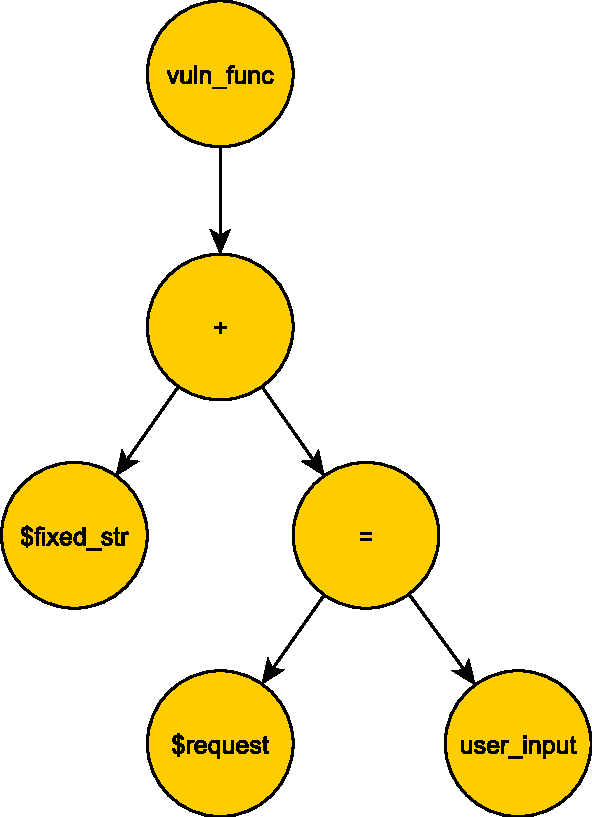
\includegraphics[max height=\textheight, max width=\textwidth]{Verwundbar_PHP_AST.pdf}
                    \captionbelow{AST des verwundbaren PHP-Skripts}\label{fig:Verwundbar_PHP_AST}
                \end{figure}

                Hierbei wurden bereits einige Vereinfachungen und
                Gruppierungen vorgenommen.

                So werden Benutzereingaben allgemein zusammengefasst als
                \lstinline{user_input} und
                potenziell verwundbare Funktionen als
                \lstinline{vuln_func}.

                Dadurch lässt sich nachvollziehen,
                wie vom Benutzer kontrollierte Eingaben in verwundbare Funktionen eingeschleust werden können.

            \subsubsection{Erkennung der Schwachstelle}\label{PHP_Erkennung der Schwachstelle}
                Die algorithmische Erkennung der Schwachstelle ist nach Erstellung des
                \gls{AST} einfach möglich:
                Eine Benutzereingabe wird ohne Filterung an eine verwundbare Funktion weitergegeben.

                Angelehnt an
                \cite[4]{Schwartz2010} wird dabei die Benutzereingabe als Quelle
                (abgeleitet vom ursprünglichen
                \foreignquote{english}{Source}) und
                die verwundbare Funktion als Senke
                (ursprünglich
                \foreignquote{english}{Sink}) bezeichnet.

                Um nun nachzuvollziehen,
                wie sich die Verunreinigung
                (ursprünglich:
                \foreignquote{english}{Taint}) fortpflanzt,
                werden in
                \vref{fig:Taint} die Knoten des
                \gls{AST} markiert,
                welche durch die Quelle verunreinigt wurden.

                \begin{figure}[htp]
                    \centering%
                    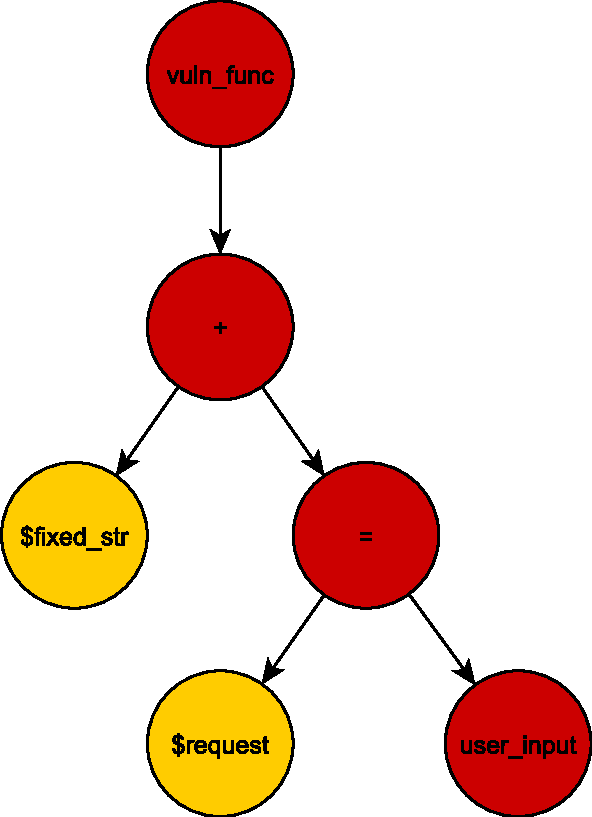
\includegraphics[max height=\textheight,
                        max width=\textwidth]{Verwundbar_PHP_AST_Taint.pdf}
                    \captionbelow{Die verunreinigten Knoten}\label{fig:Taint}
                \end{figure}

                Da in diesem Beispiel keine Filterfunktionen eingesetzt wurden,
                um die Verunreinigung zu beheben,
                kann sie sich bis zur Senke fortpflanzen.

        \subsection{Beispiel eines verwundbaren C-Programms}
            Das folgende C"=Programm ist anfällig für Buffer Overflows.

            \begin{lstlisting}[caption={Verwundbar für Buffer Overflows}, label={lst:Buffer_Overflows}, gobble=16, language=c]
                #include <stdlib.h>
                #include <unistd.h>
                #include <stdio.h>
                #include <string.h>

                int main(int argc, char **argv)
                {
                    char buffer[64];

                    gets(buffer);
                }
            \end{lstlisting}

            Für dieses Programm genügt es,
            eine Eingabe mit mehr als 64 Zeichen zu übergeben,
            um den mittels
            \lstinline{gets} befüllten Puffer auszufüllen und
            über dessen Grenzen hinaus zu schreiben.

            Das Problem hierbei ist,
            dass
            \lstinline{gets} keine Prüfung auf die Länge der Eingabe vornimmt,
            sodass es auch in der Manpage von
            \lstinline{gets} heißt:
            \foreignquote{english}{Never use gets()
            [...] it is extremely dangerous to use}
            (auf Deutsch:
            \enquote{Benutzen Sie niemals gets()
            [...] Es ist extrem gefährlich,
            es zu benutzen}).

            Die Vorgehensweise zum Ausnutzen der Sicherheitslücke wird hier aus Platzgründen nicht erläutert,
            da es sich allerdings bei dem Beispielprogramm um ein Beispiel aus der Testumgebung
            \foreignquote{english}{Protostar} von Exploit"=Exercises handelt,
            kann eine Anleitung zum Ausnutzen zum Beispiel in
            \cite{Andreko2011} gefunden werden.

            \subsubsection{Auswertung als AST}
                In diesem Fall ist die Auswertung als
                \gls{AST} noch kürzer als im Beispiel des verwundbaren
                \gls{PHP}"=Skripts,
                da die Verwendung der Funktion selbst die Schwachstelle darstellt und
                die Benutzereingabe bereits in ihr enthalten ist.

                \begin{figure}[htp]
                    \centering%
                    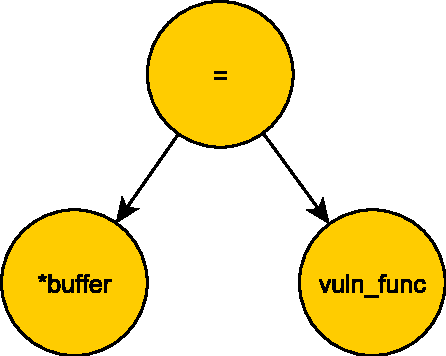
\includegraphics[max height=\textheight,
                        max width=\columnwidth]{Verwundbar_C_AST.pdf}
                    \captionbelow{AST des verwundbaren C-Programms}\label{fig:Verwundbar_C_AST}
                \end{figure}

                Als eine Besonderheit fällt auf,
                dass der
                \gls{AST} eine Zuweisung anzeigt,
                welche in dieser Form nicht explizit im Quelltext aufgeführt wird.

                Dies liegt daran,
                dass es sich bei der Variable
                \lstinline{buffer} um einen Zeiger handelt,
                woraufhin in der Funktion
                \lstinline{gets} die vom Zeiger referenzierte Speicheradresse modifiziert wird.
                Es handelt sich daher hier um eine indirekte Zuweisung,
                weshalb auch der Variablenname mit dem Dereferenzierungsoperator
                \enquote{*} gekennzeichnet wurde.

                Eine entsprechende Auflösung derartiger indirekter Zuweisungen muss daher unter Umständen auch vom Parser ermöglicht werden,
                wenn es wichtig ist zu wissen,
                ob eine Variable bei der Übergabe in eine andere Funktion kopiert wird
                (\foreignquote{english}{Call by Value}) oder
                ob sie möglicherweise auch verändert wird
                (\foreignquote{english}{Call by Reference}).

            \subsubsection{Erkennung der Schwachstelle}
                Auch in diesem Fall ist die algorithmische Erkennung der Schwachstelle einfach möglich:
                Die bloße Verwendung der
                \lstinline{gets}"=Funktion reicht aus,
                um die Schwachstelle zu ermitteln.

                \begin{figure}[htp]
                    \centering%
                    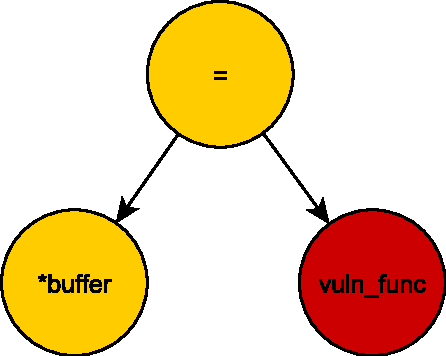
\includegraphics[max height=\textheight,
                        max width=\columnwidth]{Verwundbar_C_AST_Taint.pdf}
                    \captionbelow{Der verunreinigte Knoten}\label{fig:Taint_C}
                \end{figure}

                Entsprechend wird in
                \vref{fig:Taint_C} auch nur ein Knoten markiert,
                da keine Rückverfolgung der Quelle zur Senke notwendig ist,
                weil beides in einer Funktion liegt.

    \section{Grundprinzipien der statischen Analyse}
        Zur statischen Analyse ist,
        wie in
        \vref{PHP_Erkennung der Schwachstelle} aufgeführt,
        eine Analyse des Kontrollflusses notwendig.

        Um diese zu ermöglichen,
        sind allerdings einige Vorbereitungen notwendig.

        \begin{enumerate}
            \item Um die Unterscheidbarkeit zwischen Variablen und
              Funktionen zu gewährleisten,
              werden ihnen jeweils eindeutige Bezeichnungen zugeordnet.
            \item Da zum Beispiel die Parameter bei einer Übergabe mittels
              \foreignquote{english}{Call by Value},
              also der Übergabe von Variableninhalten durch Kopie,
              statt durch eine Übergabe des Zeigers auf den Inhalt direkt,
              unabhängig voneinander sein sollten,
              müssen gegebenenfalls zusätzliche,
              versteckte Variablen eingeführt werden,
              um die Unabhängigkeit der Inhalte zu gewährleisten.
            \item Mehrere Aufrufe einer Funktion können den Funktionsfluss ändern,
              zum Beispiel bei statischen Variablen in C oder
              Generatoren in Python.

              Um dieses Problem zu lösen,
              können Funktionen entweder kontextabhängig analysiert werden oder
              es kann versucht werden,
              diese Einschränkungen durch symbolische Ausführung bei kontextunabhängiger Analyse zu lösen.
        \end{enumerate}

        Wie aus den oben aufgeführten Problemen schnell ersichtlich wird,
        ist eine kontextunabhängige Analyse von Funktionen hinsichtlich des Implementierungsaufwands vorzuziehen und
        bringt auch nur geringe Nachteile,
        die sich durch symbolische Ausführung beheben lassen.

        Eines der Probleme bei symbolischer Ausführung besteht allerdings darin,
        dass es zu einer Explosion der möglichen Pfade durch eine Funktion kommen kann,
        wenn sämtliche Pfade probiert werden sollen.
        Eine Möglichkeit hiermit umzugehen,
        ist das Zusammenfassen ähnlicher Pfade.\cite{Kuznetsov2012}

        Eine weitere Möglichkeit,
        die in
        \vref{Vereinfachungen und deren Auswirkungen auf die Qualität der Analyse} näher beschrieben wird,
        ist es,
        Bedingungen und
        Schleifen jeweils als binäre Verzweigungen zu betrachten,
        bei denen jeder Zweig separat analysiert wird.

        Dadurch wird das Problem der Pfadexplosion ebenfalls umgangen,
        gleichzeitig ist es außerdem nicht notwendig,
        eine Zusammenfassung von Pfaden zu versuchen,
        die ebenfalls aufwendig sein kann und
        nicht immer praktikabel ist.

        Hierdurch werden zwar explizite Pfade zur Ausnutzung der Schwachstelle nicht offensichtlich und
        es kann zu mehr False Positives kommen,
        doch wird dieses Problem in Anbetracht der in
        \vref{Allgemeine Einschränkungen} beschriebenen Problematik in Kauf genommen,
        da es für eine statische Analyse auf Sicherheitslücken besser ist,
        Sicherheitslücken zu erkennen,
        deren Ausnutzung derzeit noch nicht möglich ist,
        als Sicherheitslücken zu übersehen.

    \section{Satz von Rice}\label{Satz von Rice}
        Der Satz von Rice ist ein Ergebnis aus der theoretischen Informatik und
        besagt,
        dass es keine Methode gibt,
        mit welcher man für alle Turingmaschinen verlässliche Aussagen über die von ihnen berechneten Funktionen machen kann.\cite[181]{Kuske2011}

        Informell drückt es Michael I.\ Schwartzbach,
        Professor für Informatik an der Aarhus Universität in Dänemark,
        folgendermaßen aus:
        \foreigntextquote{english}[{\cite[3]{Schwartzbach2007}}]{all interesting questions about the behavior of programs are undecidable}
        (auf Deutsch:
        \enquote{alle interessanten Fragen über das Verhalten eines Programms sind unentscheidbar}).

        Später sagt er dann über die Analyse von Datentypen:
        \foreigntextquote{english}[{\cite[7]{Schwartzbach2007}}]{Since this is an interesting question,
        we immediately know that it is undecidable.}
        (auf Deutsch:
        \enquote{Da es sich hierbei um eine interessante Frage handelt,
        wissen wir sofort,
        dass sie unentscheidbar ist.}).

        Diese Aussagen können entmutigend erscheinen.
        Die Implikationen für die statische Analyse sollen daher in
        \vref{Implikationen für die statische Analyse} näher betrachtet werden.

        Um das Problem allerdings wirklich zu verstehen,
        muss es zuerst einmal formal betrachtet werden.

        \begin{theorem}\cite[185]{Kuske2011}
            Sei \( \mathcal{R} \) die Klasse aller Turing"=berechenbaren Funktionen und
            sei \( \mathcal{S} \subseteq \mathcal{R} \) mit \( \mathcal{S} \neq \emptyset \) und
            \( \mathcal{S} \neq \mathcal{R} \).

            Dann ist die Sprache
            \[
                C(\mathcal{S}) = \{w \mid \text{die von}\ M_w\
                \text{berechnete Funktion liegt in}\ \mathcal{S}\}
            \]
            unentscheidbar.
        \end{theorem}

        \subsection{Beweis}
            Für einen einfachen Teilbeweis des Satzes von Rice reicht es bereits aus,
            ihn auf das Halteproblem zu reduzieren,
            indem man ein Programm schreibt,
            welches in Abhängigkeit des Ergebnisses des Halteproblems eine Änderung in den Eigenschaften des Programms bewirkt.

            So könnte man folgendes Programm schreiben:

            \begin{lstlisting}[caption={Das Halteproblem entscheidet über den konstanten Wert einer Variable},
                label={lst:Halteproblem_konstant}, gobble=16]
                x = 17;
                if (TM(j)) {
                    x = 18;
                }
            \end{lstlisting}

            Man sieht hieran,
            dass die Variable
            \lstinline{x} nur dann konstant ist,
            wenn die Turingmaschine
            \lstinline{j} anhält,
            was ein unentscheidbares Problem ist.\cite[3]{Schwartzbach2007}

            Natürlich ist mit diesem Teilbeweis noch nicht allgemein die Gültigkeit des Satzes von Rice bewiesen,
            auch wenn schnell ersichtlich ist,
            dass eine ähnliche Beweisführung für beliebige weitere Eigenschaften des Programms möglich wäre.

            Auf den allgemeinen Beweis des Satzes von Rice wird allerdings an dieser Stelle aus Platzgründen verzichtet,
            er kann aber in
            \cite[181-185]{Kuske2011} nachvollzogen werden.
            % Dieser einfache Beweis deckt allerdings nicht den kompletten Satz von Rice ab und
            % kann daher nur als Beispiel dienen,
            % um das Verständnis zu vereinfachen.
            % Für den strengen Beweis des Satzes ist es dagegen nötig,
            % ist es notwendig,
            % mit einem Lemma zu beginnen.
            % Der folgende Beweis entstammt XXX und
            % wird hier aber zum besseren Verständnis des Satzes von Rice in Gänze wiedergegeben.
            % \begin{lemma}
            %     Sei \( \mathcal{R} \) die Klasse aller Turing"=berechenbaren Funktionen,
            %     \( \Omega \) die nirgendwo definierte Funktion und
            %     sei \( \mathcal{S} \subseteq \mathcal{R} \) mit \( \Omega \in \mathcal{S} \) und
            %     \( \mathcal{S} \neq \mathcal{R} \).

            %     Dann ist die Sprache
            %     \[
            %         C(\mathcal{S}) = \{w \mid \text{die von}\ M_w\
            %         \text{berechnete Funktion liegt in}\ \mathcal{S}\}
            %     \]
            %     unentscheidbar.
            % \end{lemma}
            % \begin{proof}
            %     Da \( \mathcal{S} \neq \mathcal{R} \) gilt,
            %     gibt es eine Funktion \( q \in \mathcal{R} \textbackslash \mathcal{S} \).

            %     Sei \( Q \) eine Turingmaschine, die \( q \) berechnet.

            %     Wir ordnen nun jedem Wort \( w \in {\{0, 1\}}^* \) eine Turingmaschine \( M(w) \) zu,
            %     die sich bei einer Eingabe \( y \in {\{0, 1\}}^* \) wie folgt verhält:
            %     \begin{enumerate}
            %         \item \( M(w) \) ignoriert die Eingabe \( y \) zunächst und
            %               simuliert \( M_w \) auf dem leeren Band.
            %         \item Falls diese Simulation schließlich hält,
            %               so simuliert \( M(w) \) die Maschine \( Q \) auf \( y \).
            %     \end{enumerate}
            %     Dann gilt für die von \( M(w) \) berechnete Funktion \( g \):
            %     \[
            %         g = \begin{cases}
            %                 \Omega & \text{falls}\ M_w\
            %                 \text{auf dem leeren Band nicht hält,
            %                 d.\,h.}\ w \not\in H_0\\
            %                 q & \text{sonst, d.\,h.}\ w \in H_0
            %             \end{cases}
            %     \]
            %     Beachte: Es gilt \( M(w) = M_{f(w)}

            %     Dann gilt:
            %     \begin{align*}
            %         w \in H_0 &\Rightarrow g = q\\
            %                   &\Rightarrow\ \text{die von}\ M_{f(w)}\
            %                      \text{berechnete Funktion liegt nicht in}\ \mathcal{S}\\
            %                   &\Rightarrow f(w) \not\in C(\mathcal{S})
            %     \end{align*}
            %     Umgekehrt gilt auch:
            %     \begin{align*}
            %         w \not\in H_0 &\Rightarrow g = \Omega\\
            %                    &\Rightarrow\ \text{die von}\ M_{f(w)}\
            %                      \text{berechnete Funktion liegt in}\ \mathcal{S}\\
            %                    &\Rightarrow f(w) \in C(\mathcal{S})
            %     \end{align*}
            %     Es gilt also \( w \in \overline{H_0} \Leftrightarrow f(w) \in C(\mathcal{S}) \),
            %     d.\,h.\ \( \overline{H_0} \leq C(\mathcal{S}) \).
            %     Da \( H_0 \) und sein Komplement unentscheidbar sind,
            %     ist durch die Reduktion auch \( C(\mathcal{S}) \) unentscheidbar.
            % \end{proof}

            % Hiermit lässt sich nun der Satz von Rice folgendermaßen:
            % \begin{proof}
            %     Fall 1: \( \Omega \in \mathcal{S} \):
            %         Dann ist \( C(\mathcal{S}) \) nach dem eben aufgestellten Lemma unentscheidbar.

            %     Fall 2: \( \Omega \not\in \mathcal{S} \): Dann gilt
            %         \( \Omega \in \overline{S} \neq \mathcal{R} \).
            %         Nach dem eben aufgestellten Lemma ist allerdings
            %         \( C(\overline{\mathcal{S}}) \) unentscheidbar und damit auch
            %         \( C(\mathcal{S} = \overline{C(\overline{\mathcal{S}})} \).
            % \end{proof}

        \subsection{Implikationen für die statische Analyse}\label{Implikationen für die statische Analyse}
            Der Satz von Rice scheint auf den ersten Blick zu bedeuten,
            dass eine statische Analyse von Quelltexten nicht möglich ist.

            Bei näherer Betrachtung stellt sich allerdings heraus,
            dass lediglich eine eindeutige Entscheidung der Programmeigenschaften unmöglich ist.

            Dagegen ist es für die Suche nach Sicherheitslücken vollkommen ausreichend,
            eine Annäherung zu finden,
            indem nach Mustern von Schwachstellen gesucht wird.

            Mit diesen Mustern ist zum Beispiel gemeint,
            dass nach der Nutzung von bekanntermaßen verwundbaren Funktionen gesucht und
            geprüft wird,
            ob deren Eingaben vor der Nutzung korrekt abgesichert wurden.

            Eine mangelnde Absicherung würde entsprechend auf eine Sicherheitslücke hindeuten.

            Solch eine Mustersuche wird vom Satz von Rice nicht beeinträchtigt,
            allerdings wird durch ihn auf der anderen Seite klar,
            dass niemals eine in jedem Fall korrekte algorithmische statische Analyse von Quelltexten möglich sein wird.

            Eine näherungsweise Analyse mit einer gewissen Irrtumswahrscheinlichkeit ist dagegen möglich.

            Im Fall einer Schwachstellenanalyse sollte dabei versucht werden,
            den Fehler möglichst so einzugrenzen,
            dass eher False Positives,
            also Erkennung von Fehlern,
            die nicht existieren,
            als False Negatives,
            also Nichterkennung von Fehlern,
            die existieren,
            auftreten.

            Der Grund hierfür ist,
            dass sich False Positives wie
            in
            \vref{Anwendungsgebiete} beschrieben behandeln lassen,
            wohingegen es fatal sein könnte,
            Fehler im Programmcode nicht zu erkennen,
            die später zu einer Übernahme des Systems durch einen Angreifer führen können.

    \section{Graphentheorie}
        Um Quelltexte algorithmisch prüfen zu können,
        ist es notwendig,
        sie in eine abstrakte,
        für den Computer verständliche Form zu überführen.

        Hierzu wird die Graphentheorie genutzt,
        bei welcher der Zusammenhang von Objekten miteinander in einer abstrakten Struktur dargestellt wird.

        Durch die Umwandlung in diese Repräsentation kann dabei
        eine Struktur für die Speicherung der Daten abgeleitet werden.
        Weiterhin können auch Erkenntnisse aus der Graphentheorie auf die Analyse der Quelltexte angewandt werden.

        Für die Analyse von Quelltexten bietet es sich dabei an,
        die Quelltexte als eine Verbandsordnung
        (vergleiche
        \vref{Verbandsordnung}) zu betrachten,
        also eine spezielle Form der Halbordnung
        (vergleiche
        \vref{Halbordnung}).

        Aus den resultierenden vereinfachten Graphen werden im Anschluss dann Kontrollflussgraphen
        (vergleiche
        \vref{Kontrollflussgraphen}) erstellt,
        anhand derer sich nicht nur die Relation der Knoten zueinander,
        sondern auch deren Richtung bestimmen lässt.

        Hierdurch ist es schließlich möglich,
        den gesamten,
        für die Analyse notwendigen Programmablauf in einer wohldefinierten Struktur darzustellen.

        Im weiteren Verlauf wird versucht,
        die hierbei entstehenden Graphen weiter zu vereinfachen,
        um die Komplexität der folgenden Analyse zu verringern,
        und
        dabei betrachtet,
        ob diese Vereinfachung negative Auswirkungen auf das Ergebnis der Analyse haben kann.

        \subsection{Halbordnung}\label{Halbordnung}
            Eine Relation
            \( \leq \) auf einer Menge
            \( H \) ist eine Teilmenge von
            \( H \times H \).
            Wenn die folgenden Eigenschaften erfüllt sind:

            \begin{itemize}
                \item \makebox[9cm][l]{\( x \leq x \) } (Reflexivität)
                \item \makebox[9cm][l]{\( x \leq y \land y \leq x \Rightarrow x = y \)} (Antisymmetrie)
                \item \makebox[9cm][l]{\( x \leq y \land y \leq z \Rightarrow x \leq z \)} (Transitivität)
            \end{itemize}

            \( \forall\ x, y, z \in H \),
            dann ist
            \( (H, \leq) \) eine Halbordnung.\cite{Ringel2005}

            Wenn man noch einmal den
            \gls{AST} aus
            \vref{fig:Verwundbar_PHP_AST} betrachtet,
            fällt auf,
            dass hier sämtliche Eigenschaften einer Halbordnung erfüllt sind.

            In der Tat wird durch die Vorgehensweise zur Erstellung eines solchen
            \gls{AST} zwangsläufig eine Halbordnung entstehen.

            Diese Erkenntnis erlaubt es,
            entsprechende bekannte Algorithmen aus der Graphentheorie auf das Problem der statischen Analyse anzuwenden.

            Man kann die Struktur allerdings auch noch weiter spezifizieren,
            um somit weitere Spezialfälle ausnutzen zu können,
            wie im nachfolgenden Unterabschnitt gezeigt.

        \subsection{Verbandsordnung}\label{Verbandsordnung}
            Eine Verbandsordnung ist eine
            \hyperref[Halbordnung]{Halbordnung}
            \( (H, \leq) \),
            in der zu je zwei Elementen
            \( x, y \) sowohl
            \( x \lor y \),
            das Supremum,
            also die kleinste obere Schranke der Menge,
            als auch
            \( x \land y \),
            das Infimum,
            also die größte untere Schranke der Menge,
            existieren,
            wobei beide selbst nicht unbedingt Teil der Menge sein müssen.\cite{Prisner2000}

            Betrachtet man nun einen Funktionsablauf vom Start bis zum Rücksprung,
            so ergibt jeder mögliche Pfad durch diese Funktion eine Verbandsordnung,
            bei der das Supremum den Funktionsstart und
            das Infimum einen zusätzlichen
            -- nach dem ursprünglichen eingefügten
            -- Rücksprung darstellen.

            Hierdurch gelten folgende weitere Eigenschaften
            \( \forall\ x, y, z \in H \):\cite{Ringel2005}

            \begin{itemize}
                \item \makebox[9cm][l]{\( x \land x = x \), \( x \lor x = x \)} (Idempotenz)
                \item \makebox[9cm][l]{\( x \land y = y \land x \), \( x \lor y = y \lor x \)} (Kommutativität)
                \item \makebox[9cm][l]{\( (x \land y) \land c = x \land (y \land z) \), \( (x \lor y) \lor z = x \lor (y \lor z) \)} (Assoziativität)
                \item \makebox[9cm][l]{\( x \land (x \lor y) = x \), \( x \lor (x \land y) = x \)} (Absorptionsgesetz)
            \end{itemize}

        \subsection{Kontrollflussgraphen}\label{Kontrollflussgraphen}
            Ein
            \gls{CFG} ist eine Graphdarstellung sämtlicher Programmpfade während der Ausführung.
            Hierbei wird der Graph
            wie in
            \vref{Verbandsordnung} beschrieben um einen Start"= und
            einen Rücksprungknoten erweitert.

            Die Aufgabe des Kontrollflussgraphen ist es nun,
            den Programmablauf in seine Grundblöcke zu zerlegen.

            Damit sind Blöcke gemeint,
            die nur Anweisungen enthalten,
            welche direkt aufeinander folgen und
            deren Programmcode direkt hintereinandersteht.\cite[5]{Kulkarni2011}

            Als Beispiel soll der folgende Programmcode dienen:

            \begin{lstlisting}[caption={Beispiel C-Programm}, label={lst:Beispiel_C_Programm}, gobble=16, language=c]
                int a = 4,
                    b = a * 30,
                    c,
                    d = 5;
                do {
                    c = b / a;
                    if (c >= 20) {
                        d = a * c;
                    }
                } while (d < 100);
            \end{lstlisting}

            Um die Grundblöcke zu erhalten,
            müssen zuerst die Vorreiterzeilen identifiziert werden.\cite[9]{Kulkarni2011} Diese sind

            \begin{itemize}
                \item die erste Programmanweisung,
                \item explizite Ziele von Verzweigungen und
                \item implizite Ziele von Verzweigungen
            \end{itemize}

            Wenn alle Vorreiter identifiziert wurden,
            können die Basisblöcke als die Blöcke zwischen jeweils zwei Vorreitern identifiziert werden.

            Hierzu werden zuerst die Anweisungen aus
            \vref{lst:Beispiel_C_Programm} in ihre Komponenten aufgelöst:

            \begin{lstlisting}[caption={Auflösung in die Komponenten}, label={lst:Aufl_sung_in_die_Komponenten}, gobble=16, language=c]
                        int a = 4;
                        int b = a * 30;
                        int c;
                        int d = 5;
                LABEL1: c = b / a;
                        if c < 20 goto LABEL2
                        d = a * c;
                LABEL2: if d >= 100 goto LABEL3
                        goto LABEL1
                LABEL3: stop
            \end{lstlisting}

            Anschließend können gerichtete Kanten im
            \gls{CFG} erkannt werden,
            indem geprüft wird,
            ob entweder

            \begin{itemize}
                \item eine Verzweigung von der letzten Anweisung eines Basisblocks zum Vorreiter des anderen Blocks führt oder
                \item der andere Block direkt auf den ersten folgt und
                      der erste nicht in einer bedingungslosen Verzweigung endet
            \end{itemize}

            Als Resultat ergibt sich für das Programm aus
            \vref{lst:Beispiel_C_Programm} damit insgesamt der
            \gls{CFG} aus
            \vref{fig:CFG des C-Programms}.

            \begin{figure}[htp]
                \centering%
                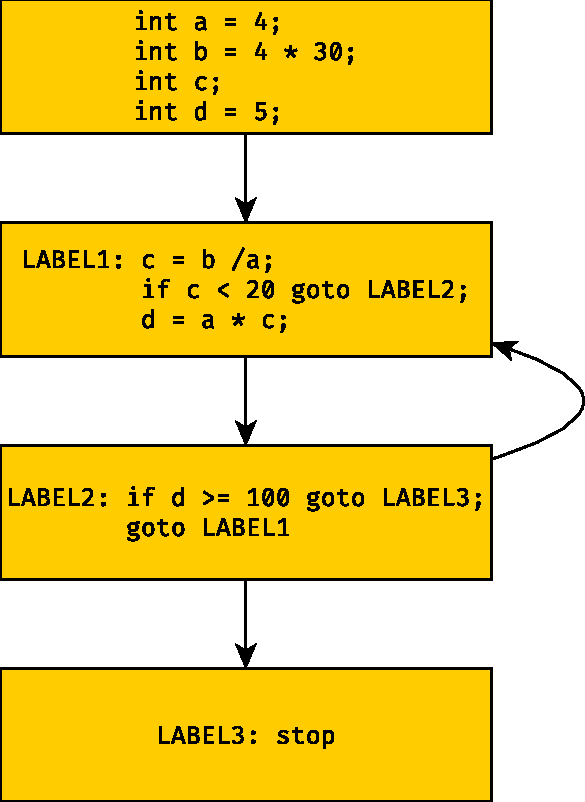
\includegraphics[max height=\textheight, max width=\columnwidth]{CFG.pdf}
                \captionbelow{CFG des C-Programms}\label{fig:CFG des C-Programms}
            \end{figure}

            Zwar ist auch eine Analyse des Kontrollflusses auf Anweisungsebene möglich,
            für die statische Suche nach Schwachstellen kann die blockbasierte Aufteilung jedoch Vorteile bringen,
            da somit der Programmablauf sehr einfach dargestellt und
            Blöcke bei Bedarf komplett ignoriert werden können,
            wenn sie keine anfälligen Anweisungen enthalten.

        \subsection{Vereinfachungen und deren Auswirkungen auf die Qualität der Analyse}\label{Vereinfachungen und deren Auswirkungen auf die Qualität der Analyse}
            Einige Vereinfachungen sind für die statische Analyse denkbar.

            Als Erstes ist es möglich,
            bei der Analyse Bedingungen und
            Schleifen jeweils als binäre Verzweigungen zu betrachten,
            bei denen jeder Zweig separat analysiert wird.

            Hierbei wird jeweils untersucht,
            ob sich die Möglichkeit einer Schwachstelle durch den betreffenden Zweig,
            unabhängig von allen anderen Verzweigungen innerhalb des Codeblocks,
            erhöht.

            Eine solche Erhöhung einer Schwachstellenwahrscheinlichkeit ergibt sich zum Beispiel,
            wenn innerhalb eines Zweiges eine Funktion aufgerufen wird,
            Während es zu einer Senkung der Schwachstellenwahrscheinlichkeit führt,
            wenn Eingaben mit festen Werten überschrieben werden,
            da hiermit ausgeschlossen wird,
            dass diese Werte benutzerkontrolliert sind oder
            bleiben.

            Hierdurch lässt sich das in
            \vref{Analyse durch symbolische Ausführung} beschriebene Problem der Pfadexplosion umgehen.
            Auf der anderen Seite ist es hierdurch aber auch denkbar,
            dass toter Code analysiert wird,
            da selbst die beiden Zweige eines
            \lstinline{if (false)} behandelt würden.
            Hierdurch könnte es zu False Positives kommen.
            Dies ist allerdings kein großes Problem,
            da
            --
            wie in
            \vref{Anwendungsgebiete} beschrieben
            -- Programme existieren,
            mit denen derartige Fehler nach einmaliger manueller Analyse von weiteren Reports ausgenommen werden können.

            Eine weitere Möglichkeit,
            die Analyse zu vereinfachen,
            ist es,
            irrelevante Codeblöcke zu ignorieren.
            Hierbei wird zuerst jeder Codeblock auf Senken untersucht und
            wenn keine gefunden wurden,
            wird der Block vorläufig zurückgestellt.
            Er wird nur dann erneut betrachtet,
            wenn in einem der darauffolgenden Blöcke eine Senke gefunden wurde.
            Sobald eine Senke gefunden wurde,
            werden die zurückgestellten Blöcke noch einmal in umgekehrter Reihenfolge untersucht,
            um die Verunreinigung zurückzuverfolgen.
            Diese Art der Vereinfachung hat keinerlei negative Auswirkungen auf die Qualität der Analyse,
            kann sie aber beschleunigen,
            da nicht mehr jeweils die gesamte Funktion,
            sondern nur noch relevante Codeblöcke mehrfach untersucht werden müssen.

    \section{Erkennung des Dateiformats}
        Bei der Suche nach Sicherheitslücken ist es wichtig zu erkennen,
        um welches Dateiformat es sich handelt.
        Ohne diese Erkennung kann nicht bestimmt werden,
        um was für eine Art von Quelltext es sich handelt
        -- oder ob es sich überhaupt um einen Quelltext handelt
        -- und
        es ist keine Erkennung von spezifischen Schwachstellen für eine Programmiersprache möglich.

        Leider ist die Erkennung des Dateiformats kein einfaches Problem,
        weshalb im Folgenden zwei gängige Methoden vorgestellt und
        miteinander verglichen werden,
        um aufzuzeigen,
        wie eine Erkennung funktionieren kann und
        welche Einschränkungen möglich sind.

        Nur wenn das Dateiformat schließlich richtig erkannt wurde,
        kann ein passendes Modul ausgewählt werden,
        durch welches das Framework eine Erkennung von Schwachstellen ermöglicht,
        indem die zu dem Modul gehörenden Regelsätze ausgewertet und
        somit sowohl Benutzereingaben,
        als auch verwundbare Funktionen erkannt werden.

        Die Erkennung des Dateiformats ist allerdings auch wichtig,
        um den richtigen Parser auszuwählen und
        somit den Inhalt der Quelltexte korrekt in einer internen Datenstruktur zu repräsentieren,
        auf der die späteren Analysen aufbauen.

        \subsection{Dateiendung}\label{Dateiendung}
            Eine auf den ersten Blick einfache Möglichkeit,
            Dateiformate korrekt zu erkennen ist es,
            die Dateiendung zu betrachten.
            Durch die Dateiendung kann ein Anwender einen Hinweis auf den Inhalt der Datei geben,
            allerdings ist die Dateiendung nicht ausschlaggebend für den Inhalt,
            da es sich hierbei lediglich um Metadaten handelt,
            die korrekt sein können oder nicht.

            So können zum Beispiel
            \gls{PNG}"=Dateien mit der Endung eines
            \gls{JPEG} abgespeichert werden,
            was von vielen Bildbetrachtungsprogrammen akzeptiert wird,
            weil beides Bildformate sind.

            Die Interpretation der Daten muss allerdings komplett unterschiedlich erfolgen,
            um erfolgreich sein zu können,
            da der interne Aufbau anders ist.

            Auf der anderen Seite können Dateiendungen auch weggelassen werden,
            wenn die Programme,
            welche die Dateien verarbeiten nicht anhand der Dateiendung,
            sondern anhand der magischen Zahl
            (vergleiche
            \vref{Magische Zahl}) versuchen,
            den Dateiinhalt zu ermitteln.

            Ein weiteres Problem bei Dateiendungen ist die Groß"= und
            Kleinschreibung.
            Während bei Windows"=Systemen die Groß"= und
            Kleinschreibung keinen Unterschied macht und
            \lstinline{test.png} und
            \lstinline{test.PNG} komplett gleich behandelt werden,
            ist diese Unterscheidung in Linux"=Systemen relevant,
            sodass eine Vereinheitlichung der Dateiendungen vor der Prüfung notwendig ist.

            Doch selbst wenn die Dateiendungen korrekt und
            in einheitlicher Schreibweise vorhanden sind,
            besteht noch das Problem,
            dass Dateiendungen nicht immer eineindeutig sind.
            So können zum einen mehrere Dateiendungen auf das gleiche Dateiformat hinweisen,
            wie zum Beispiel
            \lstinline{.cpp,.cxx,.cc,.c++,.cp,.C,.ii} für C++"=Dateien,
            wobei hier wiederum die Großschreibung von
            \lstinline{.C} wichtig ist,
            um C++"= von C"=Dateien zu unterscheiden.\cite{FSF2009}
            Zum anderen können aber auch mehrere Dateiformate für eine Dateiendung möglich sein.
            So kann eine Datei namens
            \lstinline{test.B} sowohl für einen Quelltext in
            \gls{BASIC} stehen,
            als auch für einen Quelltext in Modula"=3 oder
            einen Quelltext in den esoterischen Programmiersprachen Brainf*ck oder
            Befunge.\cite{FILExt2018}
            Selbst diese Liste ist noch nicht vollständig,
            zeigt aber das Problem,
            dass eine reine Erkennung anhand der Dateiendung zu Problemen bei der Erkennung führen könnte.

            Auf der anderen Seite kann man in den meisten Fällen davon ausgehen,
            dass die Codebasis nicht so stark durchmischt ist,
            dass es zu einer Überschneidung von Dateiformaten kommt und
            die passenden Dateiendungen im Zweifelsfall manuell eingetragen werden können.

            Eine reine Analyse der Dateiendungen ist aber aus den genannten Gründen nicht sinnvoll,
            sodass eine zusätzliche Prüfung notwendig ist,
            um entweder auch unbekannte Dateiendungen korrekt zuzuordnen
            (wenn zum Beispiel C++"=Dateien mit der Endung
            \lstinline{.cplusplus} gespeichert werden) oder
            eine eindeutige Zuordnung zu einem Dateiformat nicht möglich ist,
            wie bei den
            \lstinline{.B}"=Dateien beschrieben.

        \subsection{Magische Zahl}\label{Magische Zahl}
            Eine weitere
            -- vorwiegend im Linux"=Umfeld verbreitete
            -- Methode zur Erkennung von Dateiformaten ist die Suche nach magischen Zahlen.
            Damit ist gemeint,
            dass Dateiformate durch spezielle Zeichenketten oder
            Zahlenfolgen markiert werden,
            die anschließend mit einer Datenbank von bekannten Zahlenfolgen verglichen werden,
            um festzustellen,
            um was für ein Dateiformat es sich handelt.

            Bekannte Beispiele hierfür sind das Shebang in Shellskripten,
            \( 0\textrm{x}2321\ (8993_{10}) \)
            (\enquote{\#!}),
            wodurch angedeutet wird,
            dass die ausführbare Datei,
            die direkt im Anschluss genannt wird,
            als Interpreter für das Skript genutzt werden soll.

            Allerdings kann es auch bei der Nutzung magischer Zahlen zu Verwechslungen von Dateiformaten kommen,
            insbesondere,
            wenn es sich um kurze oder
            unvollständige Inhalte handelt,
            wie im Fall einer ausgelagerten und
            mittels
            \lstinline{#include} in C/C++ eingebundenen Anweisung,
            wie
            \vref{lst:Ausgelagert_main} und
            \vref{lst:Ausgelagert_statement} als Extrembeispiel verdeutlichen.

            \lstinputlisting[caption={Include in einer Funktion in C},
                label={lst:Ausgelagert_main}]{src/main_include.c}

            \lstinputlisting[caption={Ausgelagerte Statements in C},
                label={lst:Ausgelagert_statement}]{src/include_statement.c}

            Beide Dateien zusammen ergeben die erwartete Ausgabe
            \enquote{Testprogramm.},
            das Ergebnis des Tools
            \programname{file},
            eines traditionellen Unix"=Kommandos,
            welches anhand der magischen Zahl versucht,
            das Dateiformat einer Datei zu erkennen,
            ergibt allerdings folgende Ausgabe:

            \begin{lstlisting}[caption={Ausgabe von file}, gobble=16]
                include_statement.c: ASCII text, with CRLF line terminators
                main_include.c:      C source, ASCII text, with CRLF line terminators
            \end{lstlisting}

            Würde man sich in diesem Fall also für die Analyse nur auf die von
            \programname{file} als C"=Dateien erkannten Dateien beschränken,
            würde der Inhalt der Datei
            \filename{include\_statement.c} nicht untersucht und
            Sicherheitslücken hierin blieben unentdeckt.

            Zwar ist eine derartige Nutzung von
            \command{\#include}"=Anweisungen in der Regel eher unüblich,
            da allerdings in der Theorie beliebige Programmiersprachen durch das Framework untersucht werden können sollen,
            ist nicht auszuschließen,
            dass es Programmiersprachen gibt,
            in welchen eine derartige Herangehensweise üblich ist und
            die ebenfalls nicht korrekt durch
            \programname{file} erkannt werden würden.

            Ein weiteres Problem kann auftreten,
            wenn mehrere Dateiformate in einer Datei gemischt auftauchen,
            wie es häufiger mit
            \gls{HTML},
            \gls{CSS} und
            JavaScript der Fall ist.
            So wird die Datei aus
            \vref{lst:Multiple_Filetypes} lediglich als

            \begin{lstlisting}[gobble=16]
                multiple_filetypes.html: HTML document, ASCII text
            \end{lstlisting}

            erkannt und
            sogar bei einer Aufteilung in separate Dateien,
            wie in
            \vrefrange{lst:Separate_Filetypes}{lst:Separate_JavaScript} werden die einzelnen Dateiformate nicht korrekt erkannt:

            \begin{lstlisting}[caption={Das Resultat von file bei separaten Dateien},
                gobble=16]
                separate_css.css:        ASCII text
                separate_filetypes.html: HTML document, ASCII text
                separate_javascript.js:  ASCII text
            \end{lstlisting}

            \lstinputlisting[caption={Mehrere Dateiformate in einer Datei},
                label={lst:Multiple_Filetypes}]{src/multiple_filetypes.html}

            \lstinputlisting[caption={Separate Aufteilung in mehrere Dateien pro Dateiformat},
                label={lst:Separate_Filetypes}]{src/separate_filetypes.html}

            \lstinputlisting[caption={Separates CSS in einer Datei}]{src/separate_css.css}

            \lstinputlisting[caption={Separates JavaScript in einer Datei},
                label={lst:Separate_JavaScript}]{src/separate_javascript.js}

            Insbesondere wenn die systemeigene Magic"=Datei benutzt wird,
            kann es daher nicht nur zu für den Anwender schwer zu erkennenden Inkonsistenzen zwischen verschiedenen Systemen,
            sondern auch zu einer Nichterkennung verschiedener Dateiformate kommen,
            wodurch Sicherheitslücken in diesen übersehen werden könnten.

        \subsection{Vergleich der beiden Methoden}\label{Vergleich Dateiformaterkennung}
            Wie aus den obigen Ausführungen ersichtlich wird,
            ist keine der beiden Methoden in jedem Fall zuverlässig und
            geeignet,
            das Dateiformat immer korrekt zu erkennen.

            Um genau zu sein,
            ist eine eineindeutige Erkennung des Dateiformats auch alleine schon deshalb nicht möglich,
            weil dieselbe Datei auf unterschiedliche Arten interpretiert werden kann,
            was im einfachsten Fall durch miteinander kompatible Interpreter/Compiler zu einem ähnlichen sichtbaren Ergebnis führt,
            bei Programmiersprachen mit gleicher Syntax,
            aber unterschiedlicher Semantik jedoch zu komplett gegenläufigen Resultaten führen kann.
            Auch dieser Fall ist in der Praxis eher unüblich,
            muss jedoch für eine genaue Betrachtung beachtet und
            abgeschätzt werden,
            um die richtige Vorgehensweise zu wählen.

            Da dieses Problem durch die bloße Betrachtung des Dateinamens noch weit dramatischer ist als bei der Betrachtung der magischen Zahl,
            weil,
            wie in
            \vref{Dateiendung} beschrieben,
            die Dateiendung lediglich ein Metadatum ist,
            welches keinerlei Rückschlüsse auf den Inhalt der Datei selbst zulässt,
            sollte vorwiegend die magische Zahl zur Erkennung des Dateiformats verwendet werden.

            Um wiederum deren Schwachstellen auszugleichen,
            sollte im ersten Schritt geprüft werden,
            ob eine bekannte Dateiendung existiert und
            in diesem Fall versucht werden,
            anhand derer das Dateiformat zu erkennen,
            da erfahrungsgemäß Entwickler meistens die üblichen Dateiendungen verwenden.

            Sollte dagegen die magische Zahl keine Ergebnisse liefern und
            auch keine Dateiendung vorhanden sein,
            gibt es wiederum zwei Möglichkeiten,
            mit dem Problem umzugehen.

            Als Erstes ist es möglich,
            anhand einer Heuristik zu versuchen,
            das Dateiformat zu erraten.
            So ist davon auszugehen,
            dass in einem Verzeichnis mit mehreren hundert C++"=Dateien eine von der magischen Zahl unerkannte und
            ohne Dateiendung abgelegte Datei vermutlich am ehesten ebenfalls eine C++"=Datei sein könnte.

            Hierdurch ergibt sich wiederum die neue Frage,
            ob nur die Dateiformate der Dateien aus dem aktuellen Ordner oder
            auch die aller weiteren in die Untersuchung einbezogenen Ordner Einfluss auf die Heuristik nehmen sollten.

            Da in vielen Programmiersprachen eine Ordnung von Quelldateien in Module ordnerbasiert auf dem Dateisystem geschieht,
            werden für das Framework sämtliche untersuchten Dateien in die Heuristik einbezogen.

            Als Alternative zu dieser Heuristik muss es jedoch auch möglich sein,
            dem Framework als Anwender mitzuteilen,
            welches Dateiformat im Zweifelsfall genutzt werden soll.

            Dieses erzwungene Dateiformat würde dann die heuristische Erkennung ausschalten und
            statt dieser genutzt werden.

    \section{Erstellung von Regelsätzen}\label{Erstellung Regelsaetze}
        Die zugrunde liegenden Regelsätze sind eines der wichtigsten Kriterien,
        welche die Qualität der Erkennung beeinflussen.

        Schwachstellen,
        für die kein Regelsatz existiert,
        können von der statischen Analyse nicht korrekt als solche erkannt werden,
        wenn Regeln zu spezifisch sind,
        können leichte Abänderungen im Quelltext,
        die keine Auswirkungen auf die Sicherheit haben,
        dafür sorgen,
        dass die Erkennung fehlschlägt und
        wenn die Erstellung und
        Wartung der Regeln so aufwendig ist,
        dass nur die mitgelieferten Regeln verwendet werden,
        verliert die Analyse schnell an Bedeutung,
        da neue Angriffsmuster nicht erkannt und
        durch andere Produkte gesucht werden müssen.

        Aus diesem Grund ist es wichtig,
        zuerst zu klären,
        welchen Inhalt eine Regel überhaupt haben sollte und
        welche Details notwendig sind,
        um eine Erkennung zu gewährleisten,
        ohne die Qualität durch zu hohe Spezialisierung zu gefährden oder
        auf der anderen Seite durch zu ungenaue Regeln eine Vielzahl an Falschmeldungen zu produzieren.

        In der eigentlichen Regel müssen dann sowohl die verwundbare Funktion selbst als auch die dazu passende Absicherung enthalten sein,
        um sicherzustellen,
        dass die Zuordnung zwischen den beiden klar ist,
        da zum Beispiel die Absicherung vor
        \gls{SQL}"=Injections anders abläuft als vor
        \gls{XSS}"=Angriffen.

        Auch ist es wichtig,
        die Benutzereingaben separat zu beschreiben,
        da diese unabhängig von den verwundbaren Funktionen und
        Absicherungen sind und
        lediglich anzeigen können,
        dass die Ausnutzung durch einen Angreifer vermutlich auf direktem Weg möglich ist.

        Zudem ist wichtig festzulegen,
        ob die Regeln in einer einzelnen Datei abgespeichert werden,
        was die Installation und
        Weitergabe vereinfacht oder
        sie in mehrere Dateien aufzuteilen,
        wodurch eine einfachere Versionskontrolle der Regelsätze möglich ist.

        Auch der strukturierte Aufbau der Regeln ist wichtig,
        da die Regeln programmatisch ausgelesen und
        interpretiert werden können müssen.

        Damit Anwender später eigene Regelsätze anlegen können,
        um mit diesen ihre Quelltexte zu überprüfen,
        darf die Erstellung neuer Regeln
        -- wie bereits angesprochen
        -- ebenfalls nicht zu komplex werden.

        \subsection{Inhalt eines Regelsatzes}\label{Inhalt eines Regelsatzes}
            Im einfachsten Fall müsste ein Regelsatz lediglich Informationen darüber enthalten,
            wie eine Benutzereingabe in eine potenziell unsichere Funktion eingeschleust werden könnte und
            ob eine Absicherung der Benutzereingaben stattfindet.

            Dieser Ansatz erscheint allerdings problematisch,
            da die Auswertung der Resultate immer von einem Menschen vorgenommen werden muss.
            Aus diesem Grund erscheint es sinnvoll,
            zumindest auch eine kurze Erklärung des Regelsatzes in Form eines Kommentars zu ermöglichen.

            So könnte zu der Funktion
            \lstinline{input()} in Python ein kurzer Erklärungstext mitgegeben werden,
            dass hierdurch beliebige durch einen Zeilenumbruch begrenzte Benutzereingaben an das Programm übergeben werden können,
            wobei in Python 2 eine direkte Auswertung der Eingabe vorgenommen wird,
            sodass diese Funktion in Python 2 selbst bereits eine Sicherheitslücke darstellt.\cite{Rossum2018}

            Auch im Fall von verwundbaren Funktionen kann es wichtig sein,
            eine kurze Erklärung der Risiken mitzugeben,
            da es einem Benutzer hiermit möglich ist,
            selbst besser abzuschätzen,
            ob die Bedrohung auf das vorliegende Szenario anwendbar ist oder
            nicht.

            Weiterhin muss angegeben werden,
            ob ein spezieller Parameter der Funktion anfällig für Angriffe ist oder
            die komplette Funktion,
            wie in
            \vref{fig:Python2_input_vuln} an einem Beispiel gezeigt.

            Da Absicherungen kontextbezogen sein sollten und
            es unter Umständen nicht immer möglich ist,
            die für den konkreten Anwendungsfall korrekte Absicherung in einer Regel ausreichend zu definieren,
            kann es hilfreich sein,
            eine kurze Erklärung der Absicherung zu erlauben und
            dort aufzuschreiben,
            in welchen Szenarien sie nützlich ist.

            So ist zum Beispiel bei
            \gls{XSS}"=Injections eine Standardmethode zur Absicherung das
            \gls{HTML} Entity Encoding,
            bei dem sämtliche
            \gls{HTML}"=Zeichen in eine gleichwertige,
            aber nicht vom Browser interpretierte Darstellung umgewandelt werden.
            Diese Absicherung kann allerdings unter Umständen nicht ausreichend sein,
            wenn nur einige der Zeichen kodiert werden,
            wie zum Beispiel in Python 3s
            \lstinline{html.escape},
            welches standardmäßig nur die Zeichen
            \texttt{\&},
            \texttt{<} und
            \texttt{>} umwandelt.\cite{PSF2018a}
            Setzt man diese Kodierung allerdings in einem Kontext ein,
            in dem
            \gls{HTML}"=Attribute durch Benutzereingaben beeinflusst werden oder
            wenn man die Eingaben für
            \command{GET}"=Parameter einsetzt,
            schützt die Kodierung nicht vor Angriffen.\cite{Janca2018}

            Auch in Fällen,
            in denen eine Absicherung nicht möglich ist,
            wie bei der oben angesprochenen
            \lstinline{input}"=Funktion in Python 2 kann ein Kommentar hilfreich sein,
            der darauf hinweist,
            dass diese Funktion auf keinen Fall genutzt und
            durch die
            \lstinline{raw_input}"=Funktion ersetzt werden sollte,
            da ein Angreifer sonst recht einfach über Eingaben wie
            in
            \vref{fig:Python2_input_vuln} beliebigen Code ausführen könnte.

            \begin{figure}[htp]
                \centering%
                \includegraphics[max height=\textheight,
                    max width=\columnwidth]{Python2_input_vuln.pdf}
                \captionbelow{Die
                \command{input}"=Funktion in Python 2 erlaubt Command Injections.}\label{fig:Python2_input_vuln}
            \end{figure}

            Aus diesem Grund scheint es sinnvoll,
            zumindest noch ein optionales Kommentarfeld zu den jeweiligen Einträgen zu erlauben.

            \subsubsection{Definition von Benutzereingaben}
                Da Benutzereingaben unabhängig von verwundbaren Funktionen sind,
                müssen sie als allgemein verwendbarer Teil des jeweiligen Moduls für die einzelnen Programmiersprachen abgespeichert werden.

                Benutzereingaben werden dabei häufig über Funktionen,
                wie in
                \vref{fig:Python2_input_vuln} implementiert,
                können aber auch als Parameter beim Programmstart
                --
                wie der Parameter
                \lstinline{char* argv[]} in der
                \command{main}"=Methode von C"= und
                C++"=Programmen
                -- implementiert werden.

                Es ist hierbei wichtig zu beachten,
                dass Benutzereingaben nicht auf offensichtliche Eingaben
                wie in
                \vref{fig:Python2_input_vuln} beschränkt sind,
                sondern auch durch eingelesene Dateien,
                \gls{API}"=Schnittstellen oder
                vom Benutzer kontrollierte Umgebungsvariablen in ein Programm eingeschleust werden können.

                Die Erkennung dieser Typen von Eingaben unterscheidet sich dabei deutlich:

                \begin{enumerate}
                    \item Bei direkten Benutzereingaben muss geprüft werden,
                      ob eine entsprechende Funktion genutzt wird.
                    \item Bei eingelesenen Dateien muss geprüft werden,
                      ob der Benutzer Zugriff auf diese hat.
                    \item Bei
                      \gls{API}"=Schnittstellen müssen die Parameter einer Funktion selbst betrachtet werden.
                    \item Bei Umgebungsvariablen muss geprüft werden,
                      ob spezielle Variablen genutzt werden,
                      falls die Programmiersprache diese
                      wie im Fall von Bash und
                      anderen Skriptsprachen direkt interpretieren,
                      ohne eine entsprechende Funktion zu benötigen.
                \end{enumerate}

                Leider lassen sich nur die ersten beiden Verfahren verallgemeinern,
                indem die entsprechenden Funktionen zum Einlesen von Benutzereingaben und
                zum Öffnen bzw.\ Lesen von Dateien in einer Standardliste aufgenommen werden.

                Zusätzlich sollte daher eine projektbezogene Liste existieren,
                in der
                \gls{API}"=Schnittstellen und
                genutzte Umgebungsvariablen aufgelistet sind,
                damit auch deren Verwendung hinreichend geprüft werden kann.

                Um allerdings das Risiko durch eine fehlende Erkennung von Benutzereingaben zu senken,
                sollte die Erkennung einer Eingabe,
                die in eine verwundbare Funktion führt,
                lediglich als Erhöhung des erkannten Risikos gewertet werden und
                nicht die Voraussetzung dafür sein,
                dass die verwundbare Funktion im Risikoreport aufgeführt wird.

            \subsubsection{Definition verwundbarer Funktionen}
                Bei der Definition von verwundbaren Funktionen gibt es zwei wichtige Unterscheidungen:

                \begin{enumerate}
                    \item Funktionen,
                      die inhärent verwundbar sind,
                      wie in
                      \vref{fig:Programmablaufplan} und
                    \item Funktionen,
                      die nur dann verwundbar sind,
                      wenn an der falschen Stelle Variablen als Eingabe genutzt werden,
                      wie in
                      \vref{lst:SQL_Injections}
                \end{enumerate}

                Aus diesem Grund muss die Definition verwundbarer Funktionen es erlauben,
                nicht nur einen Funktionsnamen anzugeben,
                sondern auch,
                welcher Parameter der Funktion verwundbar ist,
                wenn er mit unkontrollierten Eingaben gespeist wird.

                So ist der folgende
                \gls{PHP}"=Code nicht verwundbar,
                obwohl die Funktion
                \lstinline{mysql_query},
                wie in
                \vref{lst:SQL_Injections} gezeigt,
                durchaus problematisch sein kann.

                \begin{lstlisting}[caption={Nicht verwundbare Nutzung von \lstinline{mysql_query}}, gobble=20, language=php]
                    mysql_query("SELECT * FROM users WHERE name = 'admin'");
                \end{lstlisting}

                Solange hier an keiner Stelle eine Benutzereingabe in die Anweisung einfließt,
                kann sie nicht direkt für Angriffe verwendet werden.

                Auf der anderen Seite ist es teilweise relevant,
                an welcher Stelle Benutzereingaben in Funktionen eingespeist werden,
                um zu unterscheiden,
                ob es sich um eine mögliche Sicherheitslücke handelt oder
                nicht.

                Als Beispiel hierfür soll die in
                \gls{PHP} 5 und
                7 vorhandene Funktion
                \lstinline{assert} dienen.\cite{PHPGroup2018}

                \begin{lstlisting}[caption={Prototyp der \lstinline{assert}-Funktion in PHP 5 und 7}, gobble=20, language=php]
                    bool assert(mixed $assertion [, string $description ])
                \end{lstlisting}

                Wird hierbei die Assertion selbst von einem Angreifer kontrolliert,
                so kann er potenziell beliebigen Code ausführen,
                wie zum Beispiel

                \begin{lstlisting}[caption={Code Execution durch Assertion}, gobble=20, language=php]
                    assert('shell_exec("uname -a"); true;');
                \end{lstlisting}

                Kontrolliert ein Angreifer dagegen nur den zweiten Parameter,
                die Beschreibung der Assertion,
                so kann er höchstens versuchen,
                seinen Text als Code in Logdateien einzuschleusen und
                darauf hoffen,
                dass das zur Betrachtung der Logdateien verwendete Programm die Einträge nicht als unsichere Eingaben behandelt,
                eine Technik,
                die allgemein als
                \foreignquote{english}{Log Poisoning} bezeichnet wird.\cite{Chandel2017}

                Derartige indirekte Angriffe können zwar ebenfalls in einen Regelsatz aufgenommen werden,
                es sollte aber hieran klar geworden sein,
                dass es einen großen Unterschied macht,
                welcher Parameter von einem Angreifer kontrolliert wird,
                um festzustellen,
                wie groß der mögliche Schaden ist.

                Die Abwehr des ersten Angriffs wird häufig auch als
                \foreignquote{english}{Output Sanitization} bezeichnet,
                womit gemeint ist,
                dass Daten vor der Weiterverwendung oder
                der Ausgabe an den Benutzer bereinigt werden,
                da die Form der Bereinigung stark von der Weiterverarbeitung abhängt.\cite{Seacord2015}

                Auf der anderen Seite würde es sich bei der Abwehr des zweiten Angriffs um eine
                \foreignquote{english}{Input Sanitization} handeln,
                also eine Bereinigung der Daten direkt nach dem Eingang,
                was nur in seltenen Fällen sinnvoll möglich ist,
                ohne die Art der Weiterverarbeitung zu kennen.\cite{Seacord2015}

                Aus diesem Grund wird die Erstellung von Regelsätzen zur
                \foreignquote{english}{Output Sanitization} empfohlen und
                es werden keine Regelsätze zur
                \foreignquote{english}{Input Sanitization} im Rahmen dieser Masterarbeit erstellt und
                mit dem Framework ausgeliefert.

            \subsubsection{Definition von Absicherungen}\label{Definition von Absicherungen}
                Absicherungen stehen vor verwundbaren Funktionen und
                sorgen dafür,
                dass die Eingaben,
                welche in die verwundbaren Funktionen eingespeist werden,
                in der verwundbaren Funktion keinen Schaden anrichten können.

                Ebenso
                wie bei der Definition verwundbarer Funktionen muss natürlich auch bei Absicherungen geprüft werden,
                welcher Parameter durch sie bereinigt wird.

                Als einfaches Beispiel sei wieder die Funktion
                \lstinline{html.escape} von Python 3 genannt.

                Wenn diese Funktion aufgerufen wird,
                bevor die Benutzereingabe in einer Webseite angezeigt wird,
                kann somit verhindert werden,
                dass Code von einem Angreifer als Code interpretiert wird und
                stattdessen durch die Umwandlung in die
                \gls{HTML} Entity Encoding der Code als Daten interpretiert wird,
                wodurch ein Angriff abgewehrt wird.

                Hierzu ergeben sich allerdings wieder einige wichtige Beobachtungen,
                ohne die eine korrekte Erkennung von Absicherungen nicht möglich ist.

                \begin{itemize}
                    \item Die verwundbare Funktion und
                      die Absicherung müssen zwingend zusammenpassen,
                      ansonsten kann die Absicherung nicht greifen,
                      wie in
                      \vref{Inhalt eines Regelsatzes} beschrieben,
                      wo der Aufruf der Funktion
                      \lstinline{html.escape} zwar im Normalfall hilft,
                      wenn komplette
                      \gls{HTML}"=Tags gefiltert werden sollen,
                      nicht mehr aber,
                      wenn auch Attribute abgesichert werden sollen.
                    \item Die Menge an Absicherungen ist nicht zwangsläufig während der kompletten Analyse konstant.
                      Dies liegt daran,
                      dass während der Analyse unter Umständen festgestellt wird,
                      dass Funktion
                      \( A \) zuerst Funktion
                      \( B \) und
                      anschließend eine verwundbare Funktion aufruft.
                      Wenn Funktion
                      \( B \) nun allerdings eine Absicherung für die in Funktion
                      \( A \) verwendete verwundbare Funktion beinhaltet und
                      so aufgerufen wird,
                      dass die Eingabe für die verwundbare Funktion in
                      \( A \) zuerst durch Funktion
                      \( B \) gefiltert wird,
                      dann ist Funktion
                      \( B \) ebenfalls eine indirekte Absicherung für die verwundbare Funktion aus
                      \( A \) und
                      muss entsprechend bewertet werden.
                \end{itemize}

                Der erste Punkt führt dazu,
                dass verwundbare Funktionen und
                zugehörige Absicherungen zwangsläufig eine gemeinsame Verbindung benötigen,
                sodass es am sinnvollsten erscheint,
                sie gemeinsam zu definieren.

                Der zweite Punkt bedeutet,
                dass ein einmaliger Scan aller Funktionen vermutlich nicht ausreichend sein wird,
                da hierdurch indirekt absichernde Funktionen nicht immer korrekt erkannt werden.

                Es ist daher notwendig,
                zuerst einen Scan auf verwundbare und
                absichernde Funktionen zu machen und
                wenn verwundbare Funktionen gefunden wurden,
                muss im nächsten Schritt geprüft werden,
                ob vor deren Aufruf in der Senke die Verschmutzung
                -- direkt oder
                indirekt
                -- abgesichert wird.

                Auf der anderen Seite kann gerade auch in der sicheren Entwicklung das Prinzip
                \foreignquote{english}{Fail Fast},
                nach dem Systeme bei Fehlern möglichst frühzeitig abbrechen sollten,
                um die Fehlererkennung zu vereinfachen und
                Fehlerfortpflanzung zu vermeiden,\cite{Shore2004}
                als Best Practice angesehen werden,
                weshalb eine Absicherung über mehrere Stufen zu einer höheren Risikoeinschätzung führen sollte,
                als eine möglichst direkte Absicherung.

                Um dies mathematisch darzustellen,
                könnte die Erkennung einer verwundbaren Funktion zuerst einen Risikofaktor von 50~Prozent bedeuten.
                Wenn zusätzlich noch eine Benutzereingabe existiert,
                deren Ergebnisse in sie eingespeist werden,
                steigt der Risikofaktor um 50 Prozentpunkte auf 100~Prozent.

                Nimmt man nun eine Absicherungsfunktion dazu,
                sollte die Risikoeinschätzung natürlich entsprechend sinken,
                zum Beispiel bei direkter Absicherung um 50 Prozentpunkte zurück auf 50~Prozent.

                Je mehr Stufen zwischen der Absicherung und
                der verwundbaren Funktion liegen,
                desto höher sollte das Risiko eingeschätzt werden.

                Für das Framework wird die folgende Funktion eingesetzt,
                sodass bei einer direkten Absicherung keine Beeinträchtigung des Risikoabfalls vorliegt,
                das Risiko aber mit steigender Anzahl indirekter Absicherungsfunktionen immer weiter wächst.

                \[ \textrm{Risiko(x)} =
                    \underbrace{0,5}_\textrm{Verwundbare Funktion} +
                    \left(\frac{
                        \min{\left(\frac{x}
                            {\underbrace{5}_\mathrm{maximale Distanz}}, 1\right)}
                        }
                        {2}\right)
                \]

                Eine grafische Darstellung dieser Funktion ist in
                \vref{fig:Wachstumsfunktion_indirekte_Absicherung} zu finden.

                \begin{figure}[htp]
                    \centering%
                    \includegraphics[max height=\textheight,
                        max width=\columnwidth]{Wachstumsfunktion_indirekte_Absicherung.PNG}
                    \captionbelow{Wachstumsfunktion für das Risiko durch indirekte Absicherung}\label{fig:Wachstumsfunktion_indirekte_Absicherung}
                \end{figure}

                Eine Benutzereingabe ohne Absicherung wird hierbei
                wie eine Absicherung mit maximaler Distanz behandelt,
                eine verwundbare Funktion ohne Benutzereingabe wie eine direkte Absicherung.

                Da eine Funktion entweder direkt aufgerufen werden kann oder
                nicht,
                ergibt sich eine Wachstumsfunktion,
                in der die Distanz als Integer übergeben wird,
                um das Risiko zu errechnen.

                Damit ergibt sich für eine Funktion,
                in der eine verwundbare Funktion mit einer Benutzereingabe aufgerufen wird und
                wo die Benutzereingabe sofort abgesichert wird,
                noch ein Restrisiko von 0,5 oder
                50~Prozent.

                Der gleiche Wert wird dadurch erreicht,
                dass eine verwundbare Funktion existiert,
                die allerdings nicht von einer Benutzereingabe betroffen ist.

                Wenn dagegen eine verwundbare Funktion mit Benutzereingabe existiert,
                deren Benutzereingabe erst in zwei Unterfunktionen bereinigt wird,
                so beträgt das Restrisiko noch 0,7 oder
                70~Prozent.

                Es ist hierbei nicht möglich,
                einen Risikowert von 0~Prozent zu erreichen,
                wenn verwundbare Funktionen genutzt werden.
                Dies ist eine bewusste Entscheidung,
                da in den meisten Fällen Alternativen existieren,
                die statt potenziell verwundbarer Funktionen eingesetzt werden sollten.

                Eine entsprechende Ab"= oder
                Aufwertung des Risikos durch weiter entfernte Benutzereingaben scheint auf der anderen Seite nicht sinnvoll.

                Um diese Entscheidung allerdings dem Benutzer zu überlassen,
                wird die maximale Entfernung als optionaler Parameter mit dem Standardwert von 5 bei der Analyse vom Benutzer abgefragt.

                Wenn keine Alternativen existieren,
                sollte den Entwicklern stets bewusst sein,
                dass sie mit der Nutzung der jeweiligen Funktion sehr vorsichtig sein müssen,
                um keine Sicherheitslücken zuzulassen.

                Auf der anderen Seite können Benutzereingaben zwar vollständig abgesichert werden,
                da jedoch die Erkennung von Benutzereingaben selbst fehleranfällig sein kann,
                kann auch eine Absicherung sämtlicher Eingaben in die verwundbare Funktion nicht dafür sorgen,
                dass die Nutzung dieser Funktion in jedem Fall sicher ist.

        \subsection{Speicherung einzelner Regeln}
            Da ein regelbasiertes Framework zur statischen Analyse in hohem Maß von der Qualität der hinterlegten Regeln abhängig ist,
            müssen alle diese Regeln betreffenden Eigenschaften genau überlegt und
            miteinander verglichen werden,
            um eine möglichst gute Lösung zu erreichen.

            Hierbei ist eine wichtige Frage,
            wie die einzelnen Regeln im Framework abgespeichert werden sollen.

            Auf der einen Seite ist die Speicherung in einer einzelnen großen Regeldatei pro Modul möglich,
            auf der anderen Seite könnte es sinnvoller sein,
            mehrere kleine Regeldateien zu erstellen,
            die unabhängig voneinander bearbeitet und
            erweitert bzw.\ wenn notwendig sogar entfernt werden können.

            Im Folgenden werden daher die Vor"= und
            Nachteile dieser beiden Methoden jeweils kurz aufgeführt und
            die beiden Ansätze miteinander verglichen.

            \subsubsection{Speicherung in einer großen Regeldatei}\label{Speicherung in einer grossen Regeldatei}
                Eine Speicherung sämtlicher Regeln in einer Datei hätte den Vorteil,
                dass der Transport dieser Datei einfacher möglich ist.

                Statt mehrere hundert kleine,
                müsste in diesem Fall nur noch eine große Datei übertragen werden,
                um Regelsätze zu aktualisieren.

                Dies hätte sowohl beim Transport selbst durch den Overhead,
                als auch beim Parsen der Dateien einen kleinen Geschwindigkeitsvorteil,
                da der Overhead in beiden Fällen einmalig wäre,
                statt bei jeder einzelnen Regeldatei aufzutreten.

                Ein weiterer Vorteil einer großen Regeldatei wäre die mögliche Kategorisierung innerhalb der Datei.
                Man könnte hier zum Beispiel einzelne Abschnitte in der Datei unterbringen,
                welche nach
                \gls{SQL}"=Injections,
                \gls{XSS}"=Schwachstellen oder
                sonstigen suchen,
                und
                müsste,
                wenn ein Treffer genauer untersucht oder
                eine Regel korrigiert werden muss,
                nur in der entsprechenden Kategorie suchen,
                um die betreffende Stelle zu finden.

                Auf der anderen Seite ist es bei großen Regeldateien schwieriger,
                Aktualisierungen nachzuvollziehen,
                wenn keine Versionsverwaltungssoftware eingesetzt wird.

                Lediglich eine große Datei zu aktualisieren könnte dafür sorgen,
                dass Benutzer gehemmt sind,
                eigene Änderungen an der Datei vorzunehmen,
                da sie befürchten müssen,
                dass ihre eigenen Änderungen an dieser beim nächsten Update überschrieben werden oder
                sie manuell die Änderungen zusammenfügen müssen.

                Weiterhin könnten sie hierdurch den Überblick über noch fehlende Regeln verlieren,
                da sie somit zwar alle Regeln auf einen Blick haben,
                aber nicht ohne weiteres sehen können,
                zu welcher Kategorie ihnen noch Regeln fehlen.

                Auch die Erweiterung um eigene Regeln würde durch eine große Regelsatzdatei erschwert,
                da die eigenen Regeln unter Umständen projektabhängig sind,
                weil zum Beispiel Frameworks eingesetzt werden,
                die ihre eigenen Funktionen zur Benutzereingabe,
                eigene verwundbare Funktionen und
                eigene Absicherungen unterstützen und
                die
                -- entweder aus Gründen der Zeitersparnis oder
                weil der Quelltext nicht vorliegt
                -- nicht bei jedem Scan mit untersucht werden sollen.

            \subsubsection{Speicherung in mehreren kleinen Dateien}
                Die Speicherung einzelner Regeln in kleinen Dateien hat den Vorteil,
                dass es sehr einfach ist,
                einzelne Regelsätze hinzuzufügen,
                Änderungen vorzunehmen und
                nachzuvollziehen und
                Regeln bei Bedarf zu entfernen.

                Auch das Debuggen von Regeln wird vereinfacht,
                wenn neben der Ausgabe der Schwachstelle auch der Name der Regeldatei,
                durch welche die Schwachstelle entdeckt wurde,
                ausgegeben wird.

                Die in
                \vref{Speicherung in einer grossen Regeldatei} angesprochenen Einbußen an Geschwindigkeit sollten vernachlässigbar sein,
                sofern es sich nicht um tausende einzelne Dateien handelt.

                Auf der anderen Seite hätte die Speicherung in Einzeldateien vor allem den Nachteil,
                dass es schwierig ist,
                einen Überblick über zu viele einzelne Dateien zu bewahren.

                Aus diesem Grund erscheint es sinnvoll,
                nicht nur ein Verzeichnis mit allen Regeldateien zu erstellen,
                sondern beliebige Unterverzeichnisse zu erlauben,
                die dann zum Beispiel thematisch geordnet sein können.

                Hiermit wäre es einem Benutzer möglich,
                schnell zwischen bestimmten Sicherheitslücken zu wechseln und
                somit gezielt nach Problemen zu suchen.

                Auch eine Einteilung nach Priorität der Schwachstelle,
                also zum Beispiel eine niedrige Priorität bei Information Disclosures,
                eine hohe Priorität bei Code Executions,
                wäre denkbar und
                könnte somit vom Benutzer frei nach den eigenen Bedürfnissen gestaltet werden.

            \subsubsection{Vergleich der beiden Ansätze}\label{Vergleich der beiden Ansätze}
                Nach Abwägung der jeweiligen Vor"= und
                Nachteile scheint es sinnvoller,
                die Regelsätze in mehrere kleine Dateien aufzuteilen,
                welche nach Bedarf in Unterverzeichnissen kategorisiert werden können.

                Eine Vorgabe für die Kategorisierung wird hierbei nicht gemacht,
                damit die Benutzer selbst die für sie optimale Kategorisierung herausfinden können.

                Hiermit lässt sich der Vorteil der großen Regeldatei
                -- die einfache Kategorisierung
                -- und
                der Vorteil der kleinen Regeldateien
                -- die bessere Änderbarkeit und
                Nachvollziehbarkeit
                -- mit minimalen Nachteilen
                -- dem Zusatzaufwand durch den Overhead vieler kleiner Dateien
                -- gut miteinander kombinieren.

        \subsection{Mögliche Formate für den Aufbau von Regeln}
            Das Format für den Aufbau von Regeln ist essenziell wichtig für den Erfolg des Projekts.

            Zuerst muss das Format in einer einheitlichen Struktur vorliegen,
            um möglichst einfach vom Framework eingelesen und
            verwertet werden zu können.

            Weiterhin ist es allerdings auch wichtig,
            dass das Format zum einen mächtig genug ist,
            um sämtliche Anforderungen,
            also die Repräsentation von Benutzereingaben
            (Quellen),
            verwundbaren Funktionen
            (Senken) und
            Absicherungen ausreichend genau darzustellen.

            Zum anderen muss es jedoch auch einfach und
            verständlich genug sein,
            dass ein typischer Benutzer in der Lage ist,
            mit möglichst wenig Einarbeitungszeit eigene Regelsätze zu erstellen oder
            vorhandene Regelsätze anzupassen.

            Außerdem steigt bei komplexeren Formaten zur Speicherung strukturierter Daten die Gefahr von Sicherheitslücken beim Parsen.

            Daher könnte ein Angreifer,
            der in der Lage ist,
            eigene Regelsätze auf einem Server zu veröffentlichen,
            eine Sicherheitslücke im Regelsatzparser ausnutzen,
            um somit die Kontrolle über den Server zu übernehmen.

            Natürlich lassen sich derartige Sicherheitslücken durch saubere Programmierung verhindern,
            die zusätzliche Komplexität der Lösung erschwert allerdings auch die Testbarkeit und
            sollte daher gut überlegt sein.

            Aus diesem Grund werden im Folgenden einige verbreitete Formate für die Speicherung strukturierter Daten vorgestellt und
            miteinander verglichen,
            um eine Lösung zu finden,
            welche sämtliche Anforderungen hinreichend erfüllt und
            dabei eine möglichst simple Struktur hat,
            sodass sie auch für unbedarfte Nutzer übersichtlich ist.

            Für einen anschaulichen Vergleich der möglichen Formate werden jeweils Beispiele für Benutzereingaben,
            verwundbare Funktionen und
            deren zugehörige Absicherungen dargestellt.

            Da davon auszugehen ist,
            dass Regelsätze auch untereinander ausgetauscht werden und
            daher nicht in jedem Fall garantiert werden kann,
            dass die Autoren vertrauenswürdig sind,
            werden auch, wo vorhanden,
            Schwachstellen und
            mögliche Sicherheitslücken durch die verschiedenen Formate aufgezeigt und
            kurz angesprochen,
            wie man diese verhindern könnte.

            Als Nebeneffekt dieser Betrachtung kann man hierdurch auch direkt weitere Regeln für die Erkennung von Schwachstellen und
            deren Absicherungen generieren,
            auch wenn die Formate nicht für die Speicherung von Regeln genutzt werden.

            \subsubsection{CSV}
                Eines der einfachsten Formate zur Speicherung strukturierter Daten,
                welches eine sehr hohe Verbreitung aufweist,
                ist das
                \gls{CSV}"=Format.

                Wie der Name bereits andeutet,
                werden hier einzelne Werte von Kommas
                (standardmäßig,
                alternativ sind auch Semikolons,
                Tabs und
                weitere Trennzeichen möglich und
                üblich) in einer Textdatei gespeichert.

                Die Einfachheit des Formats sowie
                die hohe Verbreitung sorgen hierbei dafür,
                dass eine Vielzahl an Programmen existiert,
                welche die komfortable Bearbeitung von
                \gls{CSV}"=Dateien ermöglichen.

                \gls{CSV}"=Dateien erlauben dabei eine Speicherung von Daten in einzelnen Zeilen,
                wobei jede Zeile einen separaten Datensatz darstellt.

                Optional ist auch die Speicherung von Kennungen für die einzelnen Felder in der ersten Zeile möglich.

                Durch die Trennung mit lediglich einem
                (beliebigen) Trennzeichen sind
                \gls{CSV}"=Dateien ohne dafür ausgelegte Werkzeuge ab einer bestimmten Größe nur noch mit viel Mühe lesbar.

                Weiterhin kann es zu Problemen mit Zeichensätzen,
                wechselnden Trennzeichen,
                innerhalb eines Feldes verwendeter Trennzeichen und
                leeren Feldern kommen.

                Vor allem letzteres kann problematisch werden,
                wenn mehrere optionale Felder durch nicht optionale Felder getrennt sind.
                In diesem Fall müsste das Framework raten,
                ob es sich bei dem aktuellen Feld um ein optionales Feld handelt oder
                nicht.

                \lstinputlisting[caption={Definition von Benutzereingaben für Python 3}]{src/Benutzereingaben_Python3.csv}

                \lstinputlisting[caption={Definition von verwundbaren Funktionen und Absicherungen für Python 3}]{src/Verwundbare_Funktionen_Python3.csv}

                An diesen beiden Beispielen sieht man das Format,
                in dem ein Regelsatz definiert werden kann.

                Nach einer Beschreibungszeile,
                die lediglich Metadaten enthält,
                können der Objekttyp
                -- sofern anwendbar,
                ansonsten wird das Schlüsselwort
                \lstinline{None} verwendet
                -- der Name der Funktion mit Parametern,
                der relevante Parameter für die Auswertung der Sicherheitsanalyse und
                der für die Sicherheit relevante Wert dieses Parameters und
                schließlich ein Kommentar abgespeichert werden.

                Der Objekttyp ist dabei relevant,
                um Funktionen verschiedener Objekte voneinander zu unterscheiden.
                Wenn stattdessen
                \lstinline{None} eingetragen wird,
                so wird der Objekttyp ignoriert,
                was zum Beispiel in Programmiersprachen ohne Objektorientierung sinnvoll ist.

                Beim Funktionsnamen wird der komplette Aufruf dargestellt,
                wobei optional auch Parameter mit einem vorangestellten
                \enquote{\$} markiert werden können,
                die anschließend einen festen Wert zugewiesen bekommen können,
                der für die Erkennung erforderlich ist.

                Zwischen Schrägstrichen geschriebene Werte werden als reguläre Ausdrücke erkannt,
                wie im Absicherungsparameterwert,
                in dem der Parameter
                \command{\$QUOTE} entweder mit oder
                ohne vorangestelltes
                \lstinline{quote=} stehen kann,
                wie es bei Python üblich ist,
                um Schlüsselwortargumente von positionalen Argumenten zu unterscheiden.

                Der Parameter
                \command{\$VARIABLE} stellt hierbei einen Platzhalter dar,
                in welchen die zu untersuchende Variable zur Überprüfung der Absicherung eingetragen wird.

                Um das Problem der Erkennung optionaler Felder zu behandeln,
                muss die Beschreibungszeile zwangsläufig benutzt werden,
                um dem Framework zu ermöglichen,
                fehlende Spalten korrekt zu erkennen.

                Wie bereits angesprochen ist die Verwaltung von
                \gls{CSV}"=Daten per Hand etwas mühselig,
                wie bereits an den kurzen Beispielen oben gezeigt.

                \begin{figure}[htp]
                    \centering%
                    \includegraphics[max height=\textheight, max width=\columnwidth]{Benutzereingaben_Python3.PNG}
                    \captionbelow{Definition der Benutzereingaben in Python 3 in LibreOffice}\label{fig:Benutzereingaben_Python3}
                \end{figure}

                \begin{figure}[htp]
                    \centering%
                    \includegraphics[max height=\textheight, max width=\columnwidth]{Verwundbare_Funktionen_Python3.PNG}
                    \captionbelow{Definition der verwundbaren Funktionen und deren Absicherungen in Python 3 in LibreOffice}\label{fig:Verwundbare_Funktionen_Python3}
                \end{figure}

                Allerdings lassen sich
                \gls{CSV}"=Daten auch in Programmen wie LibreOffice bearbeiten,
                wie in
                \vrefrange{fig:Benutzereingaben_Python3}{fig:Verwundbare_Funktionen_Python3} gezeigt,
                wodurch die Bearbeitung weitaus angenehmer möglich ist.

            \subsubsection{JSON}
                Ein weiteres sehr einfaches Format zur Speicherung strukturierter Daten ist
                \gls{JSON}.

                Entgegen dem Namen ist
                \gls{JSON} zwar an JavaScript angelehnt,
                kann jedoch auch in beliebigen anderen Sprachen zum Datenaustausch eingesetzt werden.

                \gls{JSON} ist dabei aussagekräftiger als
                \gls{CSV},
                da verschiedene Datentypen wie Nullwerte,
                Boolesche Werte,
                Zahlen,
                Zeichenketten,
                Arrays und
                Objekte existieren.\cite{Bray2017}

                Hierdurch ist es für automatisierte Systeme einfacher,
                die Daten korrekt zu interpretieren.

                Ein weiterer Vorteil von
                \gls{JSON} ist,
                dass die Schreibweise vergleichsweise einfach lesbar ist.

                \lstinputlisting[caption={Definition von Benutzereingaben für Python 3}]{src/Benutzereingaben_Python3.json}

                \lstinputlisting[caption={Definition von verwundbaren Funktionen und Absicherungen für Python 3}]{src/Verwundbare_Funktionen_Python3.json}

                An diesen beiden Beispielen sieht man das Format,
                in dem ein Regelsatz definiert werden kann.

                Bei dem gesamten Eintrag handelt es sich um ein Objekt,
                welches die benötigten Informationen enthält.
                Innerhalb des Objekts steht der Objekttyp,
                mit dem gearbeitet wird,
                gefolgt von einem Array aus Objekten,
                in denen die genaue Beschreibung der Benutzereingaben bzw.\ der verwundbaren Funktionen und
                deren Absicherungen stehen.

                Die Schreibweise als Array hat dabei den Vorteil,
                dass Benutzer die Möglichkeit haben,
                auch mehrere Funktionen zu definieren,
                die auf einem Objekt gefährlich sein können,
                statt pro Funktion eine eigene Regel schreiben zu müssen.

                Innerhalb des Arrays werden die Funktionen dann als ein Gesamtobjekt betrachtet,
                um zu verhindern,
                dass alle Eigenschaften als separate Einträge im Array gewertet werden.

                Das Objekt
                \lstinline{html} in der Definition der verwundbaren Funktionen und
                Absicherungen beschreibt dabei den Objekttyp der Absicherung und
                dessen Eigenschaften.

                Da eine Speicherung von regulären Ausdrücken in
                \gls{JSON} nicht vorgesehen ist,
                werden diese als Strings abgespeichert,
                welche wieder mittels
                \enquote{/} begrenzt werden,
                um anzudeuten,
                dass es sich um reguläre Ausdrücke handelt.

                Insgesamt erscheint diese Schreibweise sehr leserlich und
                weniger fehleranfällig in der Interpretation der Daten als
                \gls{CSV}.

                Für
                \gls{JSON} existiert die Erweiterung
                \gls{JSONP},
                durch die
                \gls{JSON}"=Daten über ein
                \lstinline{<script>}"=Element eingebunden und
                inklusive eines Funktionsaufrufs ausgegeben werden können.\cite{Ippolito2005}

                Diese Erweiterung ist allerdings zum einen gefährlich,
                da mit ihr Daten über Domaingrenzen hinweg ausgetauscht werden können,
                zum anderen ist sie aber auch nicht erforderlich für die Zwecke des Frameworks,
                weshalb sie,
                wenn notwendig,
                bei der Entwicklung global deaktiviert werden sollte.

            \subsubsection{YAML}\label{YAML}
                Obwohl
                \gls{JSON} einerseits besser lesbar ist als
                \gls{CSV},
                ist die Lesbarkeit doch andererseits durch einige syntaktische Eigenheiten,
                wie die Verwendung von geschweiften Klammern für Objekte und
                eckigen Klammern für Arrays sowie
                die explizite Zusammenfassung von Einträgen innerhalb eines Arrays als Objekte,
                teilweise eingeschränkt und
                kann zu Verwirrungen und Syntaxfehlern führen.

                Eine Serialisierungssprache,
                welche versucht,
                eine bessere Lesbarkeit für Menschen zu gewährleisten und
                gleichzeitig weiterhin einfach zu implementieren und
                zu nutzen zu sein,
                ist
                \gls{YAML}.

                \gls{YAML} ist dabei eine Obermenge zu
                \gls{JSON},
                was bedeutet,
                dass jedes gültige
                \gls{JSON}"=Dokument gleichzeitig auch ein gültiges
                \gls{YAML}"=Dokument ist.\cite{Ben-Kiki2009}

                Dabei versucht
                \gls{YAML} eine bessere Lesbarkeit und
                ein vollständigeres Informationsmodell zu bieten,
                indem zum Beispiel durch Erweiterungen auch das Laden von Objekten möglich ist,
                wobei Objekte sogar bei Bedarf automatisch nachgeladen werden können.

                Dies vereinfacht auf der einen Seite zwar die Speicherung von Daten und
                erlaubt einen dynamischen Inhalt von Einträgen,
                auf der anderen Seite ergeben sich allerdings hierdurch natürlich auch schwerwiegende Sicherheitslücken.

                Als Beispiel soll das Modul
                \programname{pyyaml} von Python 3 genutzt werden.

                PyYAML bietet hierbei die Funktion
                \lstinline{yaml.load} an,
                durch welche diese Erweiterung automatisch aktiviert ist.

                \begin{figure}[htp]
                    \centering%
                    \includegraphics[max height=\textheight, max width=\columnwidth]{PyYAML_verwundbar.pdf}
                    \captionbelow{PyYAMLs \lstinline{yaml.load} ist verwundbar für Code Execution}\label{fig:PyYAML_verwundbar}
                \end{figure}

                Wie in
                \vref{fig:PyYAML_verwundbar} zu sehen,
                lässt sich hierdurch von einem Angreifer,
                der Kontrolle über die
                \gls{YAML}"=Dateien hat,
                beliebiger Code ausführen.

                PyYAML bietet allerdings auch die Möglichkeit,
                mittels
                \lstinline{yaml.safe_load} nur simple Objekte
                wie Integer oder
                Listen laden zu lassen und
                weitere Objekte nur dann zuzulassen,
                wenn sie zuvor explizit im Code als
                \lstinline{yaml.SafeLoader} gekennzeichnet wurden.\cite{Net2018}

                Entsprechend müsste beim Laden von
                \gls{YAML}"=Dateien vom Framework darauf geachtet werden,
                dass nur vertrauenswürdige Objekte als Daten interpretiert werden,
                um diese Schwachstelle zu beheben.

                Als Beispiele für Regelsätze in
                \gls{YAML} werden wieder Regeln für die Erkennung von Benutzereingaben und
                für die Erkennung von verwundbaren Funktionen und
                deren Absicherungen gezeigt.

                \lstinputlisting[caption={Definition von Benutzereingaben für Python 3}]{src/Benutzereingaben_Python3.yaml}

                \lstinputlisting[caption={Definition von verwundbaren Funktionen und Absicherungen für Python 3}]{src/Verwundbare_Funktionen_Python3.yaml}

                Wie man sehen kann,
                sind die
                \gls{YAML}"=Dateien in der Tat kürzer und
                aussagekräftiger,
                als die
                \gls{JSON}"=Dateien.

                Die erhöhte Lesbarkeit durch das Python"=Objekt lässt sich allerdings bestreiten und
                erhöht die Kopplung zwischen Daten und
                Code,
                was eher hinderlich ist,
                da es zum einen Benutzer abschrecken könnte und
                zum anderen zu Verwirrung führen könnte,
                wenn Benutzer versuchen,
                eigene Funktionen zu definieren,
                die allerdings nicht korrekt funktionieren,
                wenn sie nicht als
                \lstinline{yaml.SafeLoader} definiert wurden.

                Es scheint daher sinnvoll,
                wenn
                \gls{YAML} eingesetzt werden sollte,
                die bereits in den
                \gls{CSV}"= und
                \gls{JSON}"=Dateien gezeigte Syntax für reguläre Ausdrücke zu verwenden.

                Auf der anderen Seite ist durch die Möglichkeit,
                Aliase zu definieren,
                die Gefahr gegeben,
                dass Angriffe
                wie die aus
                \gls{XML} bekannte
                \foreignquote{english}{Billion Laughs Attack} ermöglicht werden.

                So könnte das folgende
                \gls{YAML}"=Dokument zum Absturz des Parsers führen,
                da hiermit insgesamt etwa drei Gigabyte Arbeitsspeicher benötigt werden,
                um sämtliche Aliase aufzulösen.\cite{RIB2018}

                \begin{lstlisting}[caption={Billion Laughs Attacke gegen YAML}, gobble=20]
                    a: &a ["lol","lol","lol","lol","lol","lol","lol","lol","lol","lol"]
                    b: &b [*a,*a,*a,*a,*a,*a,*a,*a,*a,*a]
                    c: &c [*b,*b,*b,*b,*b,*b,*b,*b,*b,*b]
                    d: &d [*c,*c,*c,*c,*c,*c,*c,*c,*c,*c]
                    e: &e [*d,*d,*d,*d,*d,*d,*d,*d,*d,*d]
                    f: &f [*e,*e,*e,*e,*e,*e,*e,*e,*e,*e]
                    g: &g [*f,*f,*f,*f,*f,*f,*f,*f,*f,*f]
                    h: &h [*g,*g,*g,*g,*g,*g,*g,*g,*g,*g]
                    i: &i [*h,*h,*h,*h,*h,*h,*h,*h,*h,*h]
                \end{lstlisting}

                Der Angriff funktioniert hierbei so,
                dass Aliase definiert werden,
                welche sich anschließend gegenseitig referenzieren.

                Zuerst wird eine Liste
                \lstinline{a} erstellt,
                welche den Alias
                \lstinline{&a} erhält und
                aus zehn Einträgen
                \enquote{lol} besteht.
                Diese Liste wird wiederum zehnmal in Liste
                \lstinline{b} referenziert,
                die zehnmal in Liste
                \lstinline{c} referenziert wird usw.,
                sodass schlussendlich
                \( 10^9 \) Einträge entstehen,
                die insgesamt etwa drei Gigabyte Arbeitsspeicher benötigen.

                Auf der anderen Seite werden diese Aliase in PyYAML nur dann aufgelöst,
                wenn der komplette Baum durchlaufen wird,
                sodass die Gefahr als eher gering einzuschätzen ist.

                Trotzdem könnte es sinnvoll sein,
                Aliase sicherheitshalber zu deaktivieren,
                zum Beispiel durch Nutzung eines angepassten Loaders,
                wie in
                \cite{guyskk2016} zu sehen.

            \subsubsection{XML}
                Eine der am weitesten verbreiteten Serialisierungssprachen ist vermutlich
                \gls{XML}.
                Im Gegensatz zu
                \gls{YAML} versucht
                \gls{XML} dabei,
                keine reine Serialisierungssprache zu sein,
                sondern stellt eine komplette Auszeichnungssprache dar.

                Hierdurch ist
                \gls{XML} noch einmal weit mächtiger,
                als die bisher vorgestellten Formate,
                wobei allerdings fraglich ist,
                ob die zusätzlichen Möglichkeiten von
                \gls{XML} im Kontext dieses Frameworks erforderlich sind.

                Auch das Parsen von
                \gls{XML} hat
                wie schon das Parsen von
                \gls{YAML} seine Tücken,
                da es unter anderem möglich ist,
                bestehende und
                sogar externe Entitäten zu referenzieren.

                Zwei Beispiele sollen dabei diese Schwachstellen verdeutlichen.

                \begin{lstlisting}[caption={Billion Laughs-Attacke}, label={lst:Billion_Laughs_Attacke}, gobble=20]
                    <?xml version="1.0"?>
                    <!DOCTYPE lolz [
                        <!ENTITY lol "lol">
                        <!ELEMENT lolz (#PCDATA)>
                        <!ENTITY lol1 "&lol;&lol;&lol;&lol;&lol;&lol;&lol;&lol;&lol;&lol;">
                        <!ENTITY lol2 "&lol1;&lol1;&lol1;&lol1;&lol1;&lol1;&lol1;&lol1;&lol1;&lol1;">
                        <!ENTITY lol3 "&lol2;&lol2;&lol2;&lol2;&lol2;&lol2;&lol2;&lol2;&lol2;&lol2;">
                        <!ENTITY lol4 "&lol3;&lol3;&lol3;&lol3;&lol3;&lol3;&lol3;&lol3;&lol3;&lol3;">
                        <!ENTITY lol5 "&lol4;&lol4;&lol4;&lol4;&lol4;&lol4;&lol4;&lol4;&lol4;&lol4;">
                        <!ENTITY lol6 "&lol5;&lol5;&lol5;&lol5;&lol5;&lol5;&lol5;&lol5;&lol5;&lol5;">
                        <!ENTITY lol7 "&lol6;&lol6;&lol6;&lol6;&lol6;&lol6;&lol6;&lol6;&lol6;&lol6;">
                        <!ENTITY lol8 "&lol7;&lol7;&lol7;&lol7;&lol7;&lol7;&lol7;&lol7;&lol7;&lol7;">
                        <!ENTITY lol9 "&lol8;&lol8;&lol8;&lol8;&lol8;&lol8;&lol8;&lol8;&lol8;&lol8;">
                    ]>
                    <lolz>&lol9;</lolz>
                \end{lstlisting}

                Der in
                \vref{lst:Billion_Laughs_Attacke} gezeigte Angriff ist bekannt als
                \foreignquote{english}{Billion Laughs Attack} und
                stellt eine Denial of Service"=Attacke gegen den Parser dar.

                Die Funktionsweise der Attacke ist dabei identisch
                mit der
                \vref{YAML} beschriebenen.

                Um diesen Angriff abzuwehren,
                ist es möglich,
                \gls{DTD} und
                damit die Definition eigener Entitäten komplett zu unterbinden.\cite{Sullivan2009}

                Eine weitere verbreitete Attacke gegen
                \gls{XML}"=Parser ist
                \gls{XEE}.

                Hierbei wird
                --
                wie der Name bereits andeutet
                -- eine externe Entität referenziert,
                welche genutzt werden kann,
                um Daten auszuspähen oder
                ebenfalls,
                um den Parser lahmzulegen.

                \begin{lstlisting}[caption={Diese XEE legt den Parser lahm}, label={lst:XEE_urandom}, gobble=20]
                    <?xml version="1.0" encoding="ISO-8859-1"?>
                    <!DOCTYPE foo [
                        <!ELEMENT foo ANY >
                        <!ENTITY xxe SYSTEM "file:///dev/urandom" >
                    ]><foo>&xxe;</foo>
                \end{lstlisting}

                Wie in
                \vref{lst:XEE_urandom} zu sehen,
                kann durch das Einbinden von externen Entitäten eine Datei geöffnet werden,
                welche nie geschlossen wird,
                sodass der Parser endlos versucht,
                den Inhalt der Entität zu lesen.

                Ersetzt man den Pfad
                \filename{/dev/urandom} dagegen gegen
                \filename{/etc/passwd},
                so wird bei der Anzeige der Entität der Inhalt der
                \filename{/etc/passwd}"=Datei mit sämtlichen Benutzern des Systems angezeigt.\cite{Smithline2017}
                Auch dieser Angriff kann durch das Deaktivieren von
                \gls{DTD} verhindert werden.

                Wenn schließlich diese Angriffe verhindert werden,
                könnten die bekannten Regelsätze zur Erkennung von Benutzereingaben und
                verwundbaren Funktionen und
                deren Absicherungen
                wie folgt aussehen.

                \lstinputlisting[caption={Definition von Benutzereingaben für Python 3}]{src/Benutzereingaben_Python3.xml}

                \lstinputlisting[caption={Definition von verwundbaren Funktionen und Absicherungen für Python 3}]{src/Verwundbare_Funktionen_Python3.xml}

                Wie man sehen kann,
                sind die Regelsätze sehr eindeutig und
                gut lesbar.

                Auf der anderen Seite werden allerdings
                wie bei
                \gls{JSON} viele syntaktische Elemente benötigt,
                die in keinem direkten Bezug zum Inhalt der Regel stehen.

                Zwar wird hierdurch die Interpretation für den Computer vereinfacht,
                das Schreiben von Regeln wird allerdings andererseits erschwert.

            \subsubsection{Vergleich der Formate und Auswahl}\label{Vergleich der Formate und Auswahl}
                Wie man an den vorherigen Beispielen sehen kann,
                haben komplexere Formate einerseits den Vorteil,
                dass die Lesbarkeit für Mensch und
                Maschine stark verbessert wird.

                Auf der anderen Seite bieten sich aber auch immer mehr Angriffsmöglichkeiten auf den Parser derartig komplexer Sprachen.

                Im direkten Vergleich zeigt sich,
                dass subjektiv gesehen
                \gls{YAML} die beste Lesbarkeit von allen vorgestellten Formaten bietet,
                allerdings auch an einigen schwerwiegenden Sicherheitslücken leidet.

                \gls{CSV} dagegen hat die schlechteste Lesbarkeit,
                ist dafür aber auch zu simpel,
                als dass es anfällig für Sicherheitslücken wäre.

                \gls{JSON} hat eine ausreichende Lesbarkeit,
                kann aber durch Einsatz von
                \gls{JSONP} bereits zu ernsten Sicherheitsproblemen führen,
                wenn die entsprechende Erweiterung aktiviert ist.

                Auch
                \gls{XML} ist vergleichsweise ausreichend gut lesbar,
                allerdings sind die Regelsätze hier derart stark strukturiert,
                dass der Bezug zum eigentlichen Inhalt ein wenig verloren geht.
                Genau wie die anderen Formate
                -- von
                \gls{CSV} abgesehen
                -- weist
                \gls{XML} allerdings einige Sicherheitslücken auf.

                Durch die vergleichsweise beste Lesbarkeit und
                die Möglichkeit,
                die Sicherheitslücken durch entsprechende Einstellungen bzw.\ Erweiterungen abzusichern,
                fällt die Entscheidung für das Format der Regeln daher auf
                \gls{YAML}.

                Wie allerdings ebenfalls festgestellt wurde,
                führt der Einsatz regulärer Ausdrücke in den Regeln zu vielen Problemen.
                Da keine symbolische Ausführung stattfindet,
                kann hierbei nicht immer erkannt werden,
                welcher konkrete Wert während der Laufzeit wirklich eingesetzt wird.

                Entsprechend werden die Regeln so angepasst,
                dass die Parameterliste entweder den Wert
                \lstinline{null} enthalten kann,
                welcher das
                \gls{YAML}"=Äquivalent zu Pythons
                \lstinline{None} darstellt,
                oder
                den Wert
                \command{\$TAINT},
                um anzudeuten,
                dass an dieser Stelle eine benutzerdefinierte Variable eingespeist wird.

        \subsection{Erstellung universeller Regeln}
            Um die Erstellung von Regeln zu vereinfachen,
            wird im Folgenden untersucht,
            ob es möglich ist,
            universelle Regeln für die Erkennung von Schwachstellen in Quelltexten zu erstellen,
            welche unabhängig von der verwendeten Programmiersprache Sicherheitslücken erkennen.

            Eine einfache Möglichkeit wäre es,
            ein Pseudomodul hinzuzufügen,
            dessen Regeln unabhängig von der erkannten Programmiersprache
            -- und
            somit auch ohne jegliche Informationen über die Struktur dieser Sprache
            -- nach Mustern sucht,
            die als Benutzereingaben,
            Absicherungen oder
            verwundbare Funktionen erkannt werden.

            Dieser Ansatz wurde allerdings bereits in
            \vref{Einfache Stringsuche} als zu ungenau und
            aufwendig abgelehnt,
            wobei hier zusätzlich noch erschwerend hinzukommt,
            dass die Regeln sprachunabhängig sein sollten,
            wodurch sich das benötigte Muster weiter verkompliziert.

            Da dieser Ansatz keinerlei Vorteile durch die Nutzung des entwickelten Frameworks erfahren würde,
            wäre es hierbei einfacher,
            mittels spezialisierter Suchprogramme
            wie
            \gls{grep} vorzugehen.

            Eine andere Möglichkeit,
            universell einsetzbare Suchmuster für verwundbare Funktionen zu erstellen,
            wäre es,
            einen bijektiven Universalcompiler für sämtliche verwendeten Programmiersprachen zu erstellen.

            Dieser müsste nicht nur eine beliebige Programmiersprache in eine Metasprache übersetzen,
            welche anschließend auf Sicherheitslücken untersucht und
            wiederum in die ursprüngliche Programmiersprache zurück abgebildet werden können müsste,
            sondern es müssten auch Sprachkonstrukte umgewandelt und
            Abstraktionen von höheren Programmiersprachen aufgelöst werden,
            um eine Vergleichbarkeit aller Programmiersprachen zu gewährleisten.

            Eine Erstellung eines derartigen Universalcompilers ist allerdings nicht nur zum einen aus den oben genannten Gründen enorm aufwendig,
            sondern durch die Entfernung der Abstraktionen höherer Programmiersprachen fehleranfällig und
            führt zu den gleichen Schwierigkeiten,
            wie sie bei statischen Analysemethoden auf der Ebene von Binärdateien statt der eigentlichen Quelltexte auftreten.

            Wie man also sieht,
            ist die Erstellung universeller Regeln leider nicht mit vertretbarem Aufwand möglich.

    \section{Allgemeine Analyse der Codekomplexität}
        Neben der direkten Suche nach Schwachstellen im Code kann es auch sinnvoll sein,
        die Komplexität des Codes zu untersuchen,
        um zu versuchen,
        potenziell verwundbaren Code aufzuspüren.

        Die Untersuchung der Codekomplexität ist dabei kein großer zusätzlicher Aufwand,
        da bei der statischen Analyse ohnehin der komplette Code untersucht wird und
        dessen Bestandteile analysiert werden.

        Da die benutzte Metrik lediglich auf der Anzahl der Anweisungen,
        der Verzweigungen und
        der einzelnen Codeblöcke beruht,
        ist es ein Leichtes,
        diese Daten während des Scans zu erfassen und
        im Anschluss eine Bewertung auszugeben.

        Eine hohe Komplexität deutet zwar natürlich nicht automatisch auf Sicherheitslücken hin,
        wie allerdings die Kryptografen Niels Ferguson und
        Bruce Schneier schon 1999 anmerkten:
        \foreignquote{english}{Security's worst enemy is complexity}
        (auf Deutsch:
        \enquote{Komplexität ist der schlimmste Feind der Sicherheit}).\cite{Ferguson1999}

        Aus diesen Gründen erscheint es sinnvoll,
        die Codekomplexität zumindest als Resultat mit auszugeben und
        damit auf Codestellen hinzuweisen,
        welche noch einmal manuell von einem erfahrenen Programmierer auf Sicherheitslücken untersucht werden sollten.

        Da die Komplexität selbst wie
        angemerkt keine Sicherheitslücke an sich darstellt,
        sondern lediglich die Wahrscheinlichkeit für das Auftreten von Lücken erhöht,
        wird sie wertungsfrei ausgegeben,
        sofern eine bestimmte Komplexität von einer Funktion überschritten wird.

        Die zu diesem Zweck im Framework implementierte Metrik ist die von Thomas J.\ McCabe 1996 vorgestellte zyklomatische Komplexität,
        auch bekannt als die McCabe"=Metrik.

        Zwar gibt es auch noch viele weitere bekannte Metriken,
        um Codekomplexität zu messen,
        wie zum Beispiel die Halstead"=Metrik von Maurice H.\ Halstead aus dem Jahr 1977,
        allerdings sind diese zum einen aufwendiger zu messen,
        zum anderen aber sollte der Fokus des Frameworks auch nicht darauf liegen,
        komplexe Codestellen zu finden,
        was bereits eine Vielzahl anderer Programme ermöglichen,
        sondern Sicherheitslücken aufzuspüren und
        hierzu sollte es ausreichend sein,
        anhand einer Metrik auf möglicherweise zu komplexe Funktionen hinzuweisen.

        \subsection{Berechnung der McCabe-Metrik}\label{Berechnung der McCabe-Metrik}
            Die McCabe"=Metrik wird für jede Funktion berechnet als
            \( v(G) = e - n + 2 \),
            wobei
            \( e \) die Anzahl der Kanten und
            \( n \) die Anzahl der Knoten im
            \gls{CFG} darstellen.

            Zur Verdeutlichung soll ein Beispiel dienen.

            \begin{lstlisting}[caption={Der einfache euklidische Algorithmus in Python}, label={lst:Euclid}, gobble=16, language=python]
                def euclid(n, m):
                    if n > m:
                        r = m
                        m = n
                        n = r
                    r = m % n
                    while r != 0:
                        m = n
                        n = r
                        r = m % n
                    return n
            \end{lstlisting}

            \begin{figure}[htp]
                \centering%
                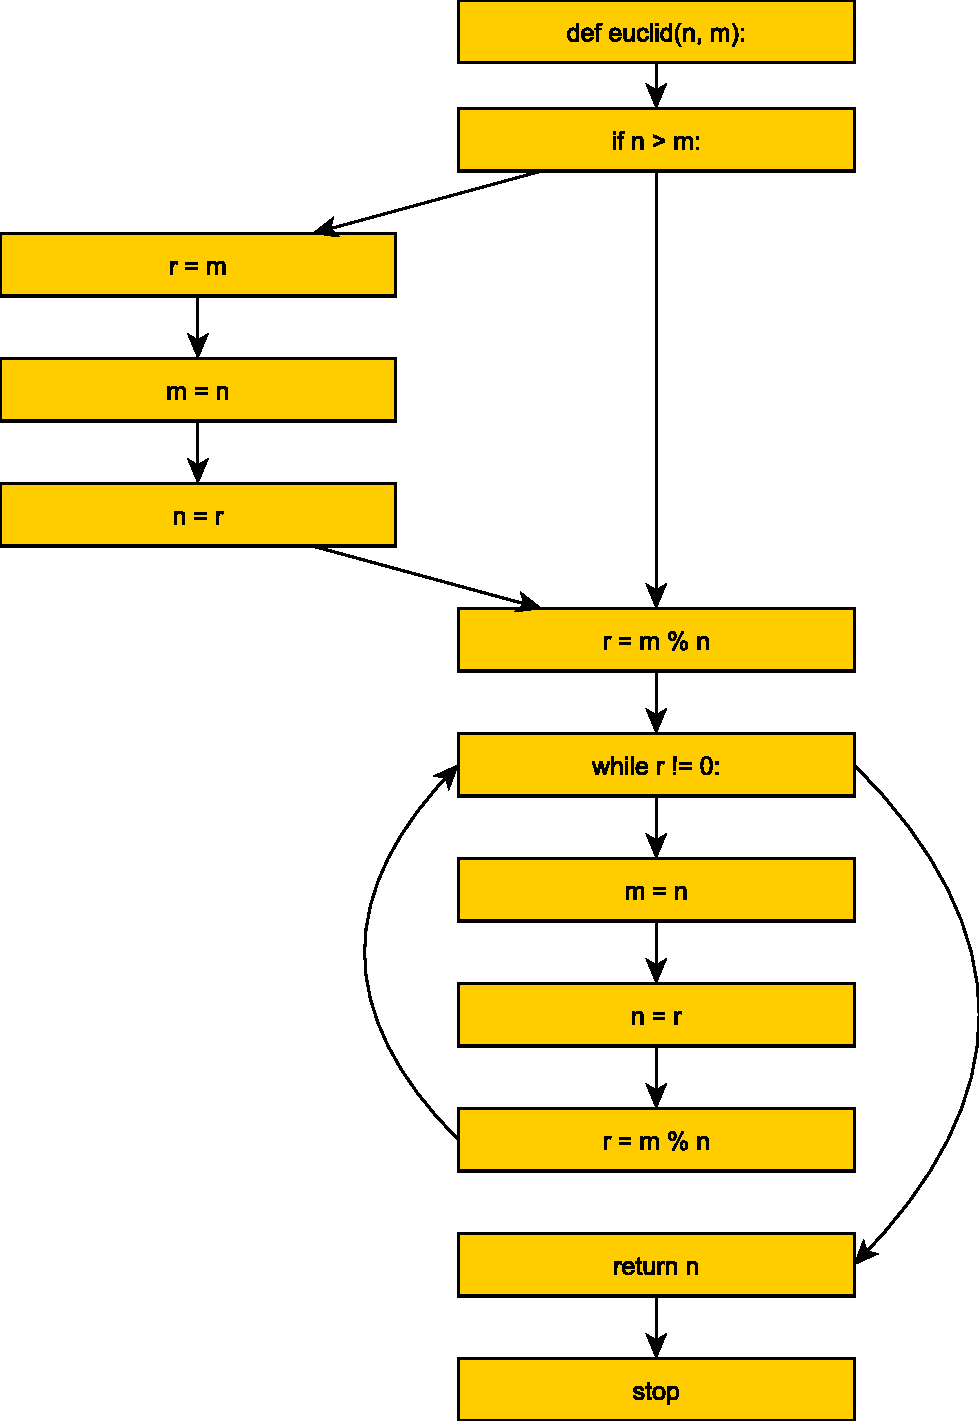
\includegraphics[max height=\textheight, max width=\columnwidth]{CFG_Euclid.pdf}
                \captionbelow{Der vollständige CFG des einfachen euklidischen Algorithmus}\label{fig:Euclid}
            \end{figure}

            Der vollständige
            \gls{CFG} zu dem Programm in
            \vref{lst:Euclid} sieht wie in
            \vref{fig:Euclid} aus.

            In diesem Fall wurden die einzelnen Anweisungen nicht in Blöcke zusammengefasst,
            da die McCabe"=Metrik jede einzelne Anweisung als einen Knoten zählt und
            somit eine Zusammenfassung das Resultat verzerren würde.

            Dem Beispiel folgend kann man sehen,
            dass in dem
            \gls{CFG} insgesamt
            \( n = 12 \) Knoten und
            \( e = 13 \) Kanten existieren,
            die sich ergebende zyklomatische Zahl ist also
            \( v(G) = 13 - 12 + 2 = 3 \).

            Hierbei ist wichtig zu beachten,
            dass sich die Anzahl der Knoten je nach Messung unterscheiden kann,
            da im ursprünglichen Paper vorgesehen ist,
            einen Pseudoknoten zwischen den Zeilen 5 und
            6 einzufügen,
            um anzudeuten,
            dass es sich bei der Verzweigung um zwei verschiedene Zweige handelt,
            selbst wenn einer der beiden komplett leer ist,
            wie in diesem Fall,
            wo der
            \lstinline{else}"=Zweig nicht explizit aufgeschrieben wurde.\cite[10]{Watson1996}

            Die meisten gängigen Testprogramme für die McCabe"=Metrik ignorieren diesen leeren Zweig,\cite{Hummel2014}
            da es allerdings für die statische Analyse erforderlich ist,
            auch leere Zweige als alternative Pfade durch eine Methode zu erkennen,
            wird für das Framework die im ursprünglichen Paper vorgeschlagene Variante genutzt.

            Der Unterschied beider Varianten ist allerdings gering genug,
            um vernachlässigbar zu sein,
            und
            da die Erkennung leerer Zweige durch die Grammatik erfolgt,
            ist es durchaus möglich,
            dass unterschiedliche Grammatiken zu unterschiedlichen Ergebnissen kommen.

            Die zyklomatische Zahl gibt für diesen Fall an,
            dass im Maximum drei Testfälle benötigt werden,
            um eine komplette Zweigüberdeckung zu erreichen,
            was als geringe Komplexität interpretiert werden kann.

            Als Faustregel gibt das Originalpaper dabei an,
            dass die zyklomatische Zahl einen Wert von 10,
            bei erfahrenen Programmierern und
            häufigen Codereviews maximal 15,
            nicht überschreiten sollte,
            da ansonsten die Komplexität zu hoch wäre,
            um noch mit vertretbarem Aufwand Testfälle zu entwerfen.\cite[25]{Watson1996}

            \subsubsection{Grundlagen der McCabe-Metrik}
                Die in der McCabe"=Metrik genutzte zyklomatische Zahl basiert auf der ersten Bettizahl.

                Bei der
                \( i \)"=ten Bettizahl eines topologischen Raums
                \( X \) handelt es sich um

                \[ b_i(X) = \dim_\mathbb{Q} H_i(X, \mathbb{Q}) \]

                für
                \( i = 0, 1, 2, \dots \),
                wobei
                \( H_i(X, \mathbb{Q}) \) die \( i \)"=te singuläre Homologiegruppe mit Koeffizienten in den rationalen Zahlen bezeichnet.\cite{Academic2015}

                Anschaulich geben die Bettizahlen an,
                wie viele
                \( k \)"=dimensionale,
                nicht zusammenhängende Flächen im topologischen Raum
                \( X \) existieren,
                sodass die erste Bettizahl,
                \( b_0 \) die Anzahl der Zusammenhangskomponenten von
                \( X \) angibt.\cite{Academic2015}

                Die erste Bettizahl eines Graphen
                \( G \) mit
                \( e \) Kanten,
                \( n \) Knoten und
                \( k \) Zusammenhangskomponenten
                ergibt dabei
                \( b_i(G) = m - n + k \),
                da das Hinzufügen einer neuen Kante entweder die Anzahl an Zusammenhangskomponenten reduziert oder
                die Anzahl an Selbstreferenzen erhöht,
                sodass das Verhältnis immer konstant bleibt.\cite{ProjectCodeMeter2014}

                Auf dieser Grundlage kann die zyklomatische Zahl berechnet werden,
                wobei als Vereinfachung bei der Berechnung der gerichtete
                \gls{CFG} als ungerichteter Graph interpretiert wird,
                da die gleiche Berechnung auch die Anzahl der unabhängigen Pfade durch einen stark zusammenhängenden gerichteten Graphen angibt.\cite[20]{Watson1996}

                Da es innerhalb einer Funktion grundsätzlich nur eine Zusammenhangskomponente geben kann,
                da die Zeilen des Quelltextes jeweils aufeinander folgen,
                kann dabei die Anzahl der Zusammenhangskomponenten
                \( k = 1 \) gesetzt werden.

                \begin{figure}[htp]
                    \centering%
                    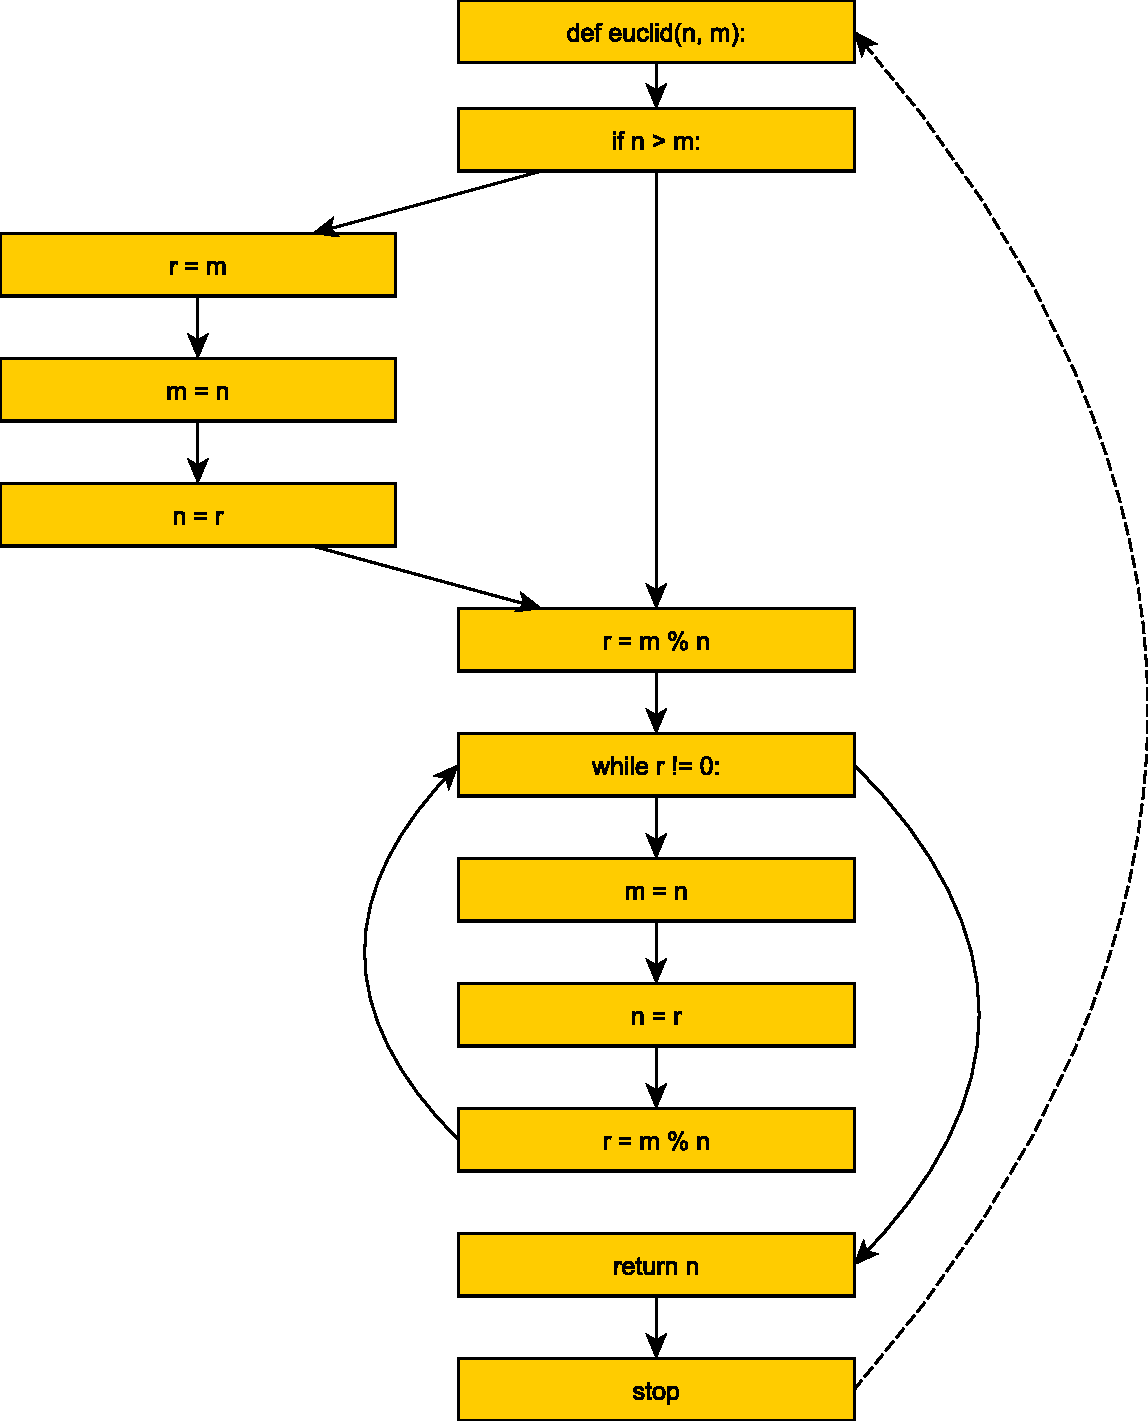
\includegraphics[max height=\textheight, max width=\columnwidth]{CFG_Euclid_virtual_backtrace.pdf}
                    \captionbelow{Der CFG wird um eine virtuelle Kante vom End- zum Startknoten erweitert}\label{fig:CFG_Euclid_virtual_backtrace}
                \end{figure}

                Allerdings stellen Programmfunktionen standardmäßig keine starken Zusammenhangskomponenten dar,
                sodass die Anzahl der Kanten um eine virtuelle Kante vom End"= zum Anfangsknoten ergänzt wird,
                wie in
                \vref{fig:CFG_Euclid_virtual_backtrace} mit einer gestrichelten Kante angedeutet.

                Insgesamt ergibt sich also für die McCabe"=Metrik hiermit die Berechnung

                \[ v(G) = e + 1 - n + \underbrace{k}_{= 1} = e - n + 2. \]

            \subsubsection{Aussagekraft}\label{Aussagekraft}
                Zwar wird die McCabe"=Metrik im Originalpaper als Methode angepriesen,
                Softwarekomplexität zu messen,\cite[5]{Watson1996}
                hierdurch werden allerdings Komplexität und
                die Anzahl der unabhängigen Wege durch ein Programm miteinander gleichgesetzt,
                was ein Trugschluss ist,
                wie im Folgenden aufgezeigt wird.

                Trotzdem wird die McCabe"=Metrik für dieses Framework eingesetzt,
                da eine direkte Messung von Softwarekomplexität nicht möglich ist und
                sich die McCabe"=Metrik trotz ihrer Schwächen als guter Indikator für Bugs in Software etabliert hat.\cite[123]{Watson1996}

                Eine dieser Schwächen,
                welche unabhängig von der Gleichsetzung von Komplexität und
                möglichen Programmpfaden ist,
                ist die unterschiedliche Messung der zyklomatischen Komplexität in verschiedenen Programmen.

                Als Beispiel hierfür kann der Code in
                \vref{lst:Euclid} gesehen werden,
                bei dem
                -- je nach Messung
                -- leere
                \lstinline{else}"=Zweige entweder als eigener Knoten gezählt werden oder
                nicht.

                Da das Originalpaper von Watson und
                McCabe aus dem Jahr 1996 stammt,
                werden weiterhin einige neuere Programmierkonzepte,
                wie Lambda"=Funktionen,
                nicht aufgeführt und
                deren Bewertung ist damit der jeweiligen Implementation überlassen.\cite{Hummel2014}

                Eine grundlegendere Schwachstelle der Metrik ist jedoch die Gleichsetzung der Pfade durch das Programm mit der Komplexität des Programms.
                Hierdurch werden zum Beispiel folgende Codes als gleichermaßen
                \enquote{kompliziert} bewertet,
                auch wenn die meisten Programmierer vermutlich anderer Ansicht sind.\cite{Hummel2014}

                \begin{lstlisting}[caption={Eine einfache Gewichtsfunktion}, gobble=20, language=java]
                    String getWeight(int i) {
                        if (i <= 0) {
                                return "no weight";
                        }
                        if (i < 10) {
                                return "light";
                        }
                        if (i < 20) {
                                return "medium";
                        }
                        if (i < 30) {
                                return "heavy";
                        }
                        return "very heavy";
                    }
                \end{lstlisting}

                \begin{lstlisting}[caption={Die Summe aller Primzahlen}, gobble=20, language=java]
                    int sumOfNonPrimes(int limit) {
                        int sum = 0;
                        OUTER: for (int i = 0; i < limit; ++i) {
                                if (i <= 2) {
                                        continue;
                                }
                                for (int j = 2; j < i; ++j) {
                                        if (i % j == 0) {
                                                continue OUTER;
                                        }
                                }
                                sum += i;
                        }
                        return sum;
                    }
                \end{lstlisting}

                Beide Codestücke haben eine zyklomatische Zahl von 5,
                allerdings ist die Komplexität der beiden stark unterschiedlich.

                Wie oben bereits angemerkt,
                existiert leider keine Metrik,
                welche die reale Komplexität von Code messen kann.

                Aus diesem Grund wird der Berechnung der McCabe"=Metrik im Kontext des Frameworks auch kein Risikowert zugewiesen,
                sondern es wird lediglich ein Hinweis auf die betroffenen Codestellen gegeben,
                sodass erfahrene Programmierer selbst prüfen müssen,
                ob die Komplexität eines Programmabschnitts zu groß ist,
                um Sicherheitslücken auszuschließen.
